\chapter{Tratamiento estadístico de datos\\ Statistical data analysis}
\chaptermark{Tratamiento de datos \textreferencemark\ Data analysis}
\epigraph{Dicen que las buenas mozas en Madrid han decidido, el gastar en vez de lengua una espada de dos filos.

Y si hay guerra en este invierno , los Valones y los Suizos llevarán en vez de espada guardapiés y rebocillo.}{El barberillo de Lavapiés. Luis Mariano de Larra}
\begin{paracol}{2}
\section{Secuencias de números aleatorios}
Se entiende por secuencia de número aleatorios, aquella en la que no es posible encontrar relación alguna entre un número de la secuencia y los que le preceden.

No es posible general secuencias de números aleatorios con un computador. La razón es que un computador es una máquina completamente determinista; la salidas que puede producir cualquier programa son completamente predecibles. Solo los procesos físicos pueden ser realmente ---intrínsecamente--- aleatorios.

Sin embargo, es posible con un ordenador generar secuencias de números que simulan ser aleatorios. Estas secuencias reciben el nombre de secuencias de números \emph{pseudoaleatorios}.\index{Números pseudoaleatorios}

El primer algoritmo para obtener números pseudoaleatorios, lo desarrolló John Von Newman en 1946. Se conoce con el nombre de \emph{Middle Square}.\index{Middle Square} La idea consiste en elegir un número inicial, formado por $n$ cifras, que recibe el nombre de semilla.\index{Números aleatorios! Semilla} A continuación se eleva el número al cuadrado. Por último, se extraen las $n$ cifras centrales del número así generado, que constituye el segundo número en la secuencia de números aleatorios. Este número se vuelve a elevar al cuadrado y se extraen de el las $n$ cifras centrales que constituirán el tercer número aleatorio. Este proceso se repite tantas veces como números aleatorios se deseen generar.

Veamos un ejemplo con una semilla  formada por $n=8$ dígitos,
\switchcolumn
\section{Random number sequences}
A random number sequence is such that it is not possible to find any relationship among a number of the sequence and the previous ones.

It is impossible to generate random numbers using a computer, because a computer is a deterministic machine and then, the outputs of any computer program are always thoroughly predictable. Only physical process could be actually --intrinsically-- unpredictable.

Nevertheless, it is possible to use the computer for generating sequences of number that seem to be random. Such sequences are called \emph{pseudo-random} number sequences.\index[eng]{Pseudo-random numbers}

The first algorithm for obtaining pseudo-random numbers was developed by John Von Newman in 1946. Its is known as the \emph{Middle Square} method. It starts from an initial number made up of n digits which is called the seed. Then, the square of the number is calculated and the n central digits of the result are taken as a new number that will be the second one of the random number sequence. This new number is squared and the n central digit of the result are taken to form the three number of the random sequence. The process is repeated so many times as random numbers you wish to generate.

Let see an example, using a n=8 digits seed, 

\end{paracol}
\begin{align*}
semilla/seed=&87289689 \rightarrow
87289689^2={\color{red}7619}\ 48980571\ {\color{red}6721}\\
&48980571\rightarrow
48980571^2={\color{red}2399}\ 09633548\ {\color{red}6041}\\
&09633548 \rightarrow
09633548^2={\color{red}0092}\ 80524706\ {\color{red}8304}\\
&80524706 \rightarrow
80524706^2={\color{red}6484}\ 22827638\ {\color{red}6436}\\
&22827638\\
&\ \ \ \ \ \vdots
\end{align*}
\begin{paracol}{2}
El siguiente código de Python, permite obtener una lista de números pseudoaleatorios mediante el método \emph{Middle Square}
\switchcolumn
The next Python code allows us to get a list a pseudo-random number using the Middle Square method,
\end{paracol}

\inputminted[
frame=lines,
framesep=2mm,
baselinestretch=1.2,
%bgcolor=LightGray,
label=middlesquare.py,
fontsize=\footnotesize,
linenos
]{python}{./codigos/tratamiento_datos/middlesquare.py}

\begin{paracol}{2}
Las secuencias generadas mediante el método \emph{middle square} no son aleatorias, cada número viene completamente determinado por el número anterior. Sin embargo, dichas secuencias parecen aleatorias. La figura \ref{fig:middlesquare} muestra una secuencia de $100$ valores pseudoaleatorios generados mediante \emph{middle square}. Aparentemente, cada valor parece no guardar ninguna relación con los anteriores.

El método descrito, presenta sin embargo serios inconvenientes: Si la semilla contiene ceros o unos a la derecha, estos tienden a repetirse indefinidamente. Además todos los métodos inducen ciclos que hacen que los números generados comiencen a repetirse periódicamente. Por ejemplo, si empezamos con la semilla de cuatro dígitos $3708$,  La secuencia cae, tras generar los primeros cuatro números aleatorios, en un ciclo en el que los cuatro siguientes números generados se repiten indefinidamente.

\switchcolumn
Sequences generated using the middle square method are not random, each number is thoroughly determined by the previous one. Nevertheless, these sequences seems random. Figure \ref{fig:middlesquare} shows a sequence of 100 pseudo-random values generated using the middle square. Apparently, each value doesn't seem to have any relationship with the previous ones.

However, this method has significant drawbacks: if the seed contains zeros or ones on the right side, these values tend to repeat indefinitely. Besides, all methods induce cycles, which make the generated numbers begin to repeat periodically. For instance, If we begin with the four-digit seed $3708$, The sequence gets into a cycle after it generates the first four random numbers. The four subsequent numbers repeat indefinitely.
\end{paracol}
\begin{figure}[h]
	\centering
	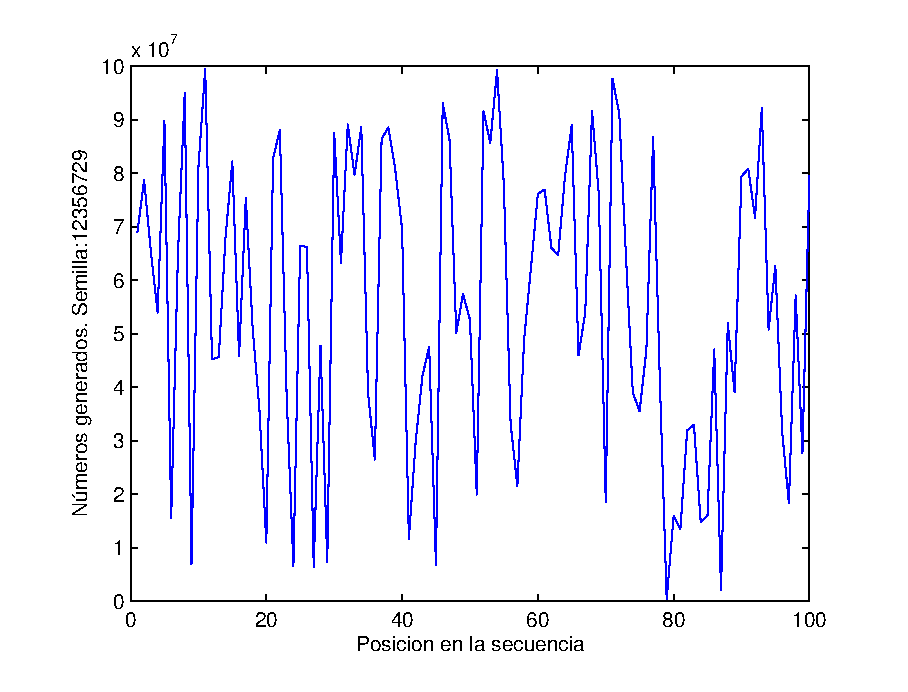
\includegraphics[width=12cm]{middlesquare.eps}
	\bicaption{Secuencia de $100$ números pseudoaleatorios generada mediante el método \emph{middle square}.}{$100$ pseudo-random numbers sequence generates using the \emph{middle square} method}
	\label{fig:middlesquare}
\end{figure}
\begin{align*}
semilla/seed=3708 \rightarrow
&3708^2={\color{red}13}\ 7492\ {\color{red}64}\\
&7492^2={\color{red}56}\ 1300\ {\color{red}64}\\
&1300^2={\color{red}01}\ 6900\ {\color{red}00}\\
&6900^2={\color{red}47}\ 6100\ {\color{red}00}\\
&6100^2={\color{red}37}\ 2100\ {\color{red}00}\\
&2100^2={\color{red}04}\ 4100\ {\color{red}00}\\
&4100^2={\color{red}16}\ 8100\ {\color{red}00}\\
&8100^2={\color{red}65}\ 6100\ {\color{red}00}\\
&6100^2={\color{red}37}\ 2100\ {\color{red}00}\\
&2100^2={\color{red}04}\ 4100\ {\color{red}00}\\
&4100^2={\color{red}16}\ 8100\ {\color{red}00}\\
&\ \ \ \vdots
\end{align*}

\begin{paracol}{2}
Además, en la secuencia generada puede observarse cómo los ceros situados a las derecha una vez que aparecen en la secuencia, se conservan siempre.

En los algoritmos de generación de números aleatorios, la idea es obtener números en el intervalo $[0,1]$. Para ello, se generan números entre $0$ y un número natural $m$ y luego se dividen los números generados, $X_n$ entre $m$,
\switchcolumn
Besides, it is possible to see how the the zeros locate at the right size, once they turn up, remain for ever.

Algorithms for random number generation are usually designed to generate numbers in the interval $[0,1]$. This is carried out generating a number between $0$ an a natural number $m$ and, after, dividing the generated numbers $X_n$ by $m$,  
\end{paracol}

\begin{equation*}
U_n=\frac{X_n}{m}
\end{equation*}

\begin{paracol}{2}
Usualmente, se elige para $m$ un valor tan grande como sea posible. 
En 1948 Lehmer propuso un algoritmo conocido con el nombre de \emph{linear congruential}. El algoritmo emplea cuatro elementos numéricos,

\begin{itemize}
\item[-] $I_0$, Semilla. Análoga a la del método \emph{middle square}.
\item[-] $m > I_0$, Módulo.  Se elige tan grande como sea posible. Cuanto mayor es el módulo, mayor es el periodo del ciclo inducido.
\item[-] $a$, Multiplicador. Debe elegirse de modo que $0\le a < m$
\item[-] $c$, Incremento. Debe elegirse de modo que $0\le c < m$
\end{itemize}
 
El algoritmo de obtención de la secuencia de números pseudoaleatorios se define en este caso como,

\switchcolumn
Usually, a value as large as possible is chosen for $m$. In 1948 Lehmmer proposed an algorithm known as \emph{linear congruential}. This algorithm uses four numerical items,

\begin{itemize}
	\item[-] $I_0$, Seed. Similar to \emph{middle square} method.
	\item[-] $m > I_0$, modulus.  it is chossen as large as posible. The larger the modulus the lager the period of the induced cycle.
	\item[-] $a$, Multiplier. Should be chosen to meet that $0\le a < m$
	\item[-] $c$, Increment. Should be chosen to meet that $0\le c < m$
\end{itemize}
 
 Then, the algorithm to obtain the sequence of random number is defined as,
\end{paracol}

\begin{equation*}
I_{n+1}=\text{rem}(a\cdot I_n+c, m)
\end{equation*}

\begin{paracol}{2}
Es decir, cada número se obtiene como el resto de la división entera del producto del multiplicador por el número aleatorio anterior más el incremento, divido entre el módulo. Por tanto, se trata de un número comprendido entre $0$ y $m-1$. 

El siguiente código permite calcular una secuencia de números aleatorios por el método \emph{linear congruential}

\switchcolumn
Each number is calculated as the remainder of the product of the multiplier and the previous random number, added to the increment, all divided by the modulus. This results in a number between 0 and m-1.

The following code calculates a sequence of random numbers using the \emph{linear congruential} method. 
\end{paracol}
\inputminted[
frame=lines,
framesep=2mm,
baselinestretch=1.2,
%bgcolor=LightGray,
label=linearcong.py,
fontsize=\footnotesize,
linenos
]{python}{./codigos/tratamiento_datos/linearcong.py}

\begin{paracol}{2}
Una variante del algoritmo descrito, frecuentemente empleada, se obtiene haciendo el incremento igual a cero, $c=0$. Dicha variante se conoce con el nombre de \emph{multiplicative congruential}, su expresión general sería,
\switchcolumn
We can get a frequently used variation of the linear congruential algorithm taking the increment equal to zero, $c=0$. Such variation is known as the \emph{multiplicative congruential} algorithm; a general expression for it would be, 
\end{paracol}
\begin{equation*}
I_{n+1}=\text{rem}(a\cdot I_n)
\end{equation*}
\begin{paracol}{2}
Dado que el resto de la división entera de un número cualquiera entre el módulo $m$ solo puede tomar valores enteros comprendidos entre $0$ y $m-1$, es fácil deducir que, en el mejor de los casos, podríamos obtener un ciclo de longitud $m$, antes de que secuencia de números aleatorios comenzara a repetirse. De ahí la importancia de elegir $m$ lo más grande posible. Por otra parte, los valores de $I_0$ e $c$, también influyen en la longitud de los ciclos inducidos.

Si ahora dividimos los numero aleatorios obtenidos por el modulo,  
\switchcolumn


Since the integer division of whatever number by the modulus $m$ can yield results between $0$ and $m-1$, it becomes clear that, in the best-case scenario, we can achieve a cycle of length $m$ before the sequence of random numbers starts to repeat. Hence, the importance of choosing a large as possible value for $m$. On the other hand, the values taken by $I_0$ and $c$ also influence the length of the induced cycles.

If we now divide the random number achieved by the modulus,
\end{paracol}
\begin{equation*}
x_n=\frac{I_n}{m} \Rightarrow x_n \in [0,1]
\end{equation*}

\begin{paracol}{2}
Los números así obtenidos pertenecen al intervalo $[0,1]$ y están regularmente distribuidos. 

En la década de los 60 del siglo pasado, La compañía IBM, desarrolló una función, conocida como \emph{Randu}, que utilizaba el algoritmo \emph{multiplicative congruential}. \emph{Randu} tenía definido un multiplicador $c=2^{16}+3$ y un módulo $m=2^{31}$. 
Se han desarrollado diferentes variante de \emph{Randu}, mejorando progresivamente su rendimiento. Una de las mejoras introducidas fue aumentar el número de semillas empleadas,

\switchcolumn
The number obtained belong to the interval $[0,1]$ and are regularly distributed.

In the last century sixties, IBM company developed a function known as \emph{Randu} which employed the \emph{multiplication congruential} algorithm. \emph{Randu} had defined a multiplier $c=2^{16}+3$ and modulus $m=2^{31}$.
Several variations of \emph{Randu} have been developed, gradually improving its performance. One of these improvements was to increase the number of seeds the algorithm uses.  
\end{paracol}
\begin{equation*}
I_{n+1}=\text{rem}(a\cdot I_n+b\cdot I_{n-1}+\cdots)
\end{equation*} 
\begin{paracol}{2}
Este método permite obtener periodos mayores.
\switchcolumn
This method leads to get longer periods
\end{paracol}

\subsection{El generador de números aleatorios de Matlab.}\label{rand} Se trata de un generador mucho mas evolucionado que los ejemplo descritos hasta ahora.  La implementación concreta depende de la versión de Matlab empleada. Aquí solo nos referiremos a la conocida como \emph{'twister'}. Se basa en el algoritmo \emph{Mersenne Twister}. Genera números aleatorios, uniformemente distribuidos, en el intervalo $[2^{-53}, 1-2^{-53}] $. El periodo de la secuencia generada es $P=(2^{19937}-1)/2$. Es el algoritmo que emplea Matlab, por defecto, desde al versión 2007 hasta la actualidad.

Para generar números aleatorios se emplea el comando \texttt{rand}, que es capaz de generar una matriz de tamaño arbitrario de números aleatorios.  Si se invoca el comando \texttt{rand}, sin indicar ninguna variable de entrada, 
\begin{verbatim}
>> y=rand
y =
     8.147236863931789e-01
\end{verbatim}
Matlab nos devuelve un único número aleatorio. Si introducimos un único valor entero como variable de entrada,
\begin{verbatim}
>> x=rand(3)
x =
     9.057919370756192e-01     6.323592462254095e-01     5.468815192049838e-01
     1.269868162935061e-01     9.754040499940952e-02     9.575068354342976e-01
     9.133758561390194e-01     2.784982188670484e-01     9.648885351992765e-01
\end{verbatim}
Obtenemos una matriz cuadra de números aleatorios cuyas dimensiones coinciden con el número entero introducido. 

Si empleamos dos enteros como variables de entrada, \texttt{rand(f,c)}, obtenemos una matriz de números aleatorios de dimensión $f\times c$.
\begin{verbatim}
>> x=rand(3,2)
x =
     7.922073295595544e-01     3.571167857418955e-02
     9.594924263929030e-01     8.491293058687771e-01
     6.557406991565868e-01     9.339932477575505e-01
\end{verbatim}

Cada vez que se arranca Matlab, el generador de números aleatorios es reiniciado. Es decir, cada vez que arrancamos Matlab, volvemos a obtener la misma secuencia de números aleatorios. Podemos hacer que el generador se reinicie siempre que queramos, empleado para ello una semilla constituida por un número entero que debe estar comprendido entre $0$ y $2^{32}-1$. Para cada semilla obtendremos una secuencia de números distinta. Para reiniciar el generador, empleamos  la función \texttt{rng} y el valor de la semilla. Por ejemplo,
\begin{verbatim}
>> rng(10)
\end{verbatim}

Si generamos ahora una secuencia de 3 números aleatorios,
\begin{verbatim}
>> s1=rand(1,3)
s1 =
    0.7713    0.0208    0.6336
\end{verbatim}
Si reiniciamos de nuevo el algoritmo, con la misma semilla de antes y volvemos a generar una secuencia de 3 números aleatorios,
\begin{verbatim}
>> rnd(10)
>> s1=rand(1,3)
s1 =
    0.7713    0.0208    0.6336
\end{verbatim}
Volvemos a obtener los mismo números aleatorios. Esto sucederá siempre que reiniciemos el generador empleado la misma semilla.

Por ultimo, podemos emplear \texttt{rng} para conoces el estado del generador de números aleatorios en cualquier momento, durante una sesión con Matlab. Para ello, usamos \texttt{rng} Sin ninguna variable de entrada,
\begin{verbatim}
estado=rnd
\end{verbatim}
El resultado es:
\begin{verbatim}
estado = 
  struct with fields:

     Type: 'twister'
     Seed: 10
    State: [625x1 uint32]
\end{verbatim}
Nos devuelve el generador utilizado para obtener los números aleatorios, la semilla, en este caso \texttt{twister}, La semilla empleada para inicializar el generador y un vector de 625 enteros que son las semillas que el generador empleará para generar el siguiente número aleatorio.

Si queremos cambiar el generador de números aleatorios empleado por matlab, empleamos de nuevo la función rnd, indicando un valor para la semilla y el nombre del generador entre comillas\footnote{Para obtener una relación completa de generadores, consultar la ayuda de matlab},
\begin{verbatim}
>> rng(0,'philox')
>> estado = rng
estado = 
  struct with fields:

     Type: 'philox'
     Seed: 0
    State: [7x1 uint32]
\end{verbatim}

Supongamos que después de obtener el estado del generador, seguimos generando números aleatorios. Podemos hacer que el generador vuelva al estado que tenía empleando la estructura obtenida para leinicializar el generador. A partir de ahí el generador volverá a repetir de nuevo la misma secuencia de números aleatorios. La siguiente secuencia de instrucciones de Matlab ilustra este procedimiento,
%\begin{lstlisting}
%% ejemplo de vuelta del generador de numeros aleatorios a un estado
%% anterior
%
%% generamos una secuencia de 5 números,
%s1=rand(1,5)
%% guardamos el estado actual del generador
%estado=rng;
%
%% generamos una nueva secuencia de 5 números
%s2=rand(1,5)
%
%% volvemos a llevar el generador al estado anterior,
%rng(estado)
%
%% volvemos a generar una secuencia de 5 números que será igual que s2
%s2bis=rand(1,5)
%\end{lstlisting}

Si ejecutamos la secuencia obtendremos,

\begin{verbatim}
s1 =
    0.3655    0.6975    0.1789    0.4549    0.4396

s2 =
     0.5174    0.7001    0.4564    0.7388    0.4850
      
s2bis =
    0.3655    0.6975    0.1789    0.4549    0.4396
\end{verbatim}

Por último podemos reiniciar el generador empleando,
\begin{verbatim}
>> rng('shuffle')
\end{verbatim}
En este caso, matlab suministra una semilla obtenida a partir de la hora actual.

\section{Probabilidad y distribuciones de probabilidad}

La probabilidad es una propiedad asociada a los sucesos aleatorios. Decimos que un suceso es aleatorio cuando no depende de una causa determinista que nos permite predecir cuándo va a suceder. \index{Suceso Aleatorio}

\subsection{Sucesos aleatorios discretos}
Por ejemplo, obtener \emph{cara} o \emph{cruz} al lanzar una moneda al aire es un ejemplo sencillo de proceso aleatorio, ya que no es posible conocer de antemano cuál será el resultado del lanzamiento. La probabilidad da una medida de las posibilidades de que un determinado suceso aleatorio tenga lugar.

Volviendo al ejemplo de la moneda  lanzada al aire, las posibilidades son dos:
\begin{enumerate}
\item Que salga cara.
\item Que salga cruz.
\end{enumerate}
Ambos sucesos son igualmente probable tras un lanzamiento, uno de los dos debe darse necesariamente y no hay, en principio, ningún otro suceso posible. Podemos entonces asociar valores numéricos a la probabilidad con la que se dan las distintas posibilidades:
\begin{itemize}
\item La probabilidad de que salga cara o cruz ---cualquiera de las dos--- debe tener asociado el valor máximo ya que \emph{necesariamente} ha de salir cara o cruz.  Habitualmente se toma como valor máximo de un suceso aleatorio el valor $1$, que estaría asociado con el suceso necesario o cierto,
\begin{equation*}
P(\text{cara o cruz}) = 1
\end{equation*}

\item La probabilidad de que no salga ni cara ni cruz. Puesto que hemos establecido que ha de salir necesariamente cara o cruz, estamos ante un suceso imposible. A los sucesos imposibles se les asigna probabilidad $0$,
\begin{equation*}
P(\emptyset) = 0
\end{equation*}

\item La probabilidad de que salga cara. Como en una moneda cara y cruz son igualmente probables,  la probabilidad de sacar cara, sera la \emph{mitad} de la probabilidad de sacar cara o cruz,
\begin{equation*}
P(\text{cara})=\frac{1}{2}=0.5
\end{equation*}

\item La probabilidad de sacar cruz. De modo análogo al caso anterior será la mitad de la probabilidad de sacar cara o cruz, 

\begin{equation*}
P(\text{cara})=\frac{1}{2}=0.5
\end{equation*} 
\end{itemize}

\begin{figure}
\centering
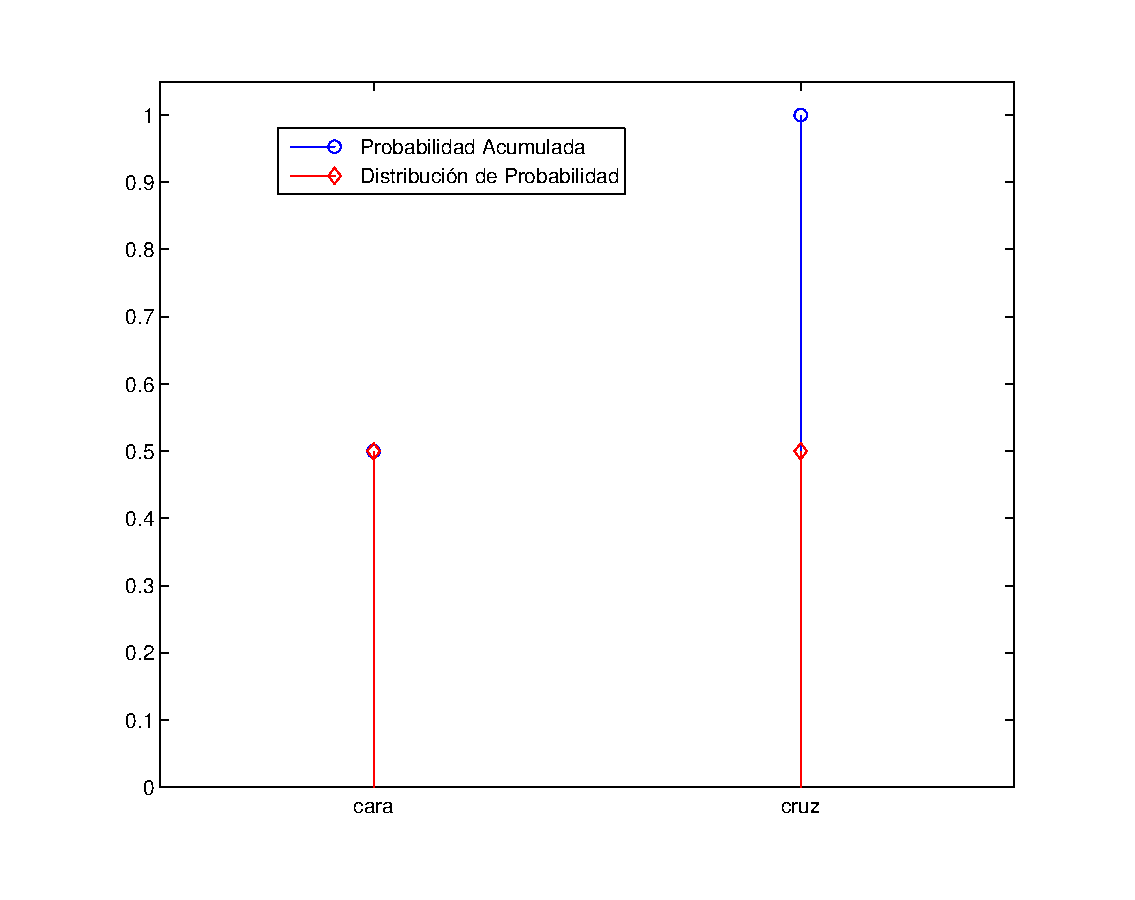
\includegraphics[width=10cm]{probcaracruz.eps}
\caption{Distribución de probabilidad y probabilidad acumulada de los resultados de lanzar una moneda al aire.}
\label{fig:moneda}
\end{figure}


Lanzar una moneda o un dado, elegir una carta al azar, rellenar una quiniela, son ejemplos de fenómenos aleatorios discretos. Reciben este nombre, porque los sucesos posibles asociados al fenómeno son numerables, es decir, se pueden contar.  Así por ejemplo en el lanzamiento de una moneda solo hay dos sucesos posibles (cara o cruz), en el de un dado hay seis (cada una de sus caras), en el de la elección de una carta hay cuarenta (si se trata de una baraja española) etc. El conjunto de sucesos posibles recibe el nombre de variable aleatoria. \index{Variable! aleatoria}

Una distribución de probabilidad discreta, es una función que asocia cada caso posible de un fenómeno aleatorio con su probabilidad. Si vamos sumando sucesivamente las probabilidades de todos los fenómenos posibles, lo que obtenemos es una nueva función que recibe el nombre de probabilidad acumulada (Más adelante volveremos sobre esta idea). La figura \ref{fig:moneda} muestra la distribución de probabilidad y la probabilidad acumulada asociadas al lanzamiento de una moneda al aire.

Si todos los sucesos posibles dentro de un fenómeno aleatorio discreto tienen la misma probabilidad de suceder,  es posible determinar directamente la probabilidad de cada uno de ellos sin más que  dividir los casos favorables  entre los casos posibles,

\begin{equation*}
P(a)=\frac{\text{casos en que se da} \ a}{\text{numero total de casos posibles}}
\end{equation*}

Así por ejemplo la probabilidad de sacar un $6$ cuando se laza un dado será,

\begin{equation*}
P(a)=\frac{\text{casos en que se da}\ a=1}{\text{numero total de casos posibles}=6}=\frac{1}{6}
\end{equation*}

\begin{figure}
\centering
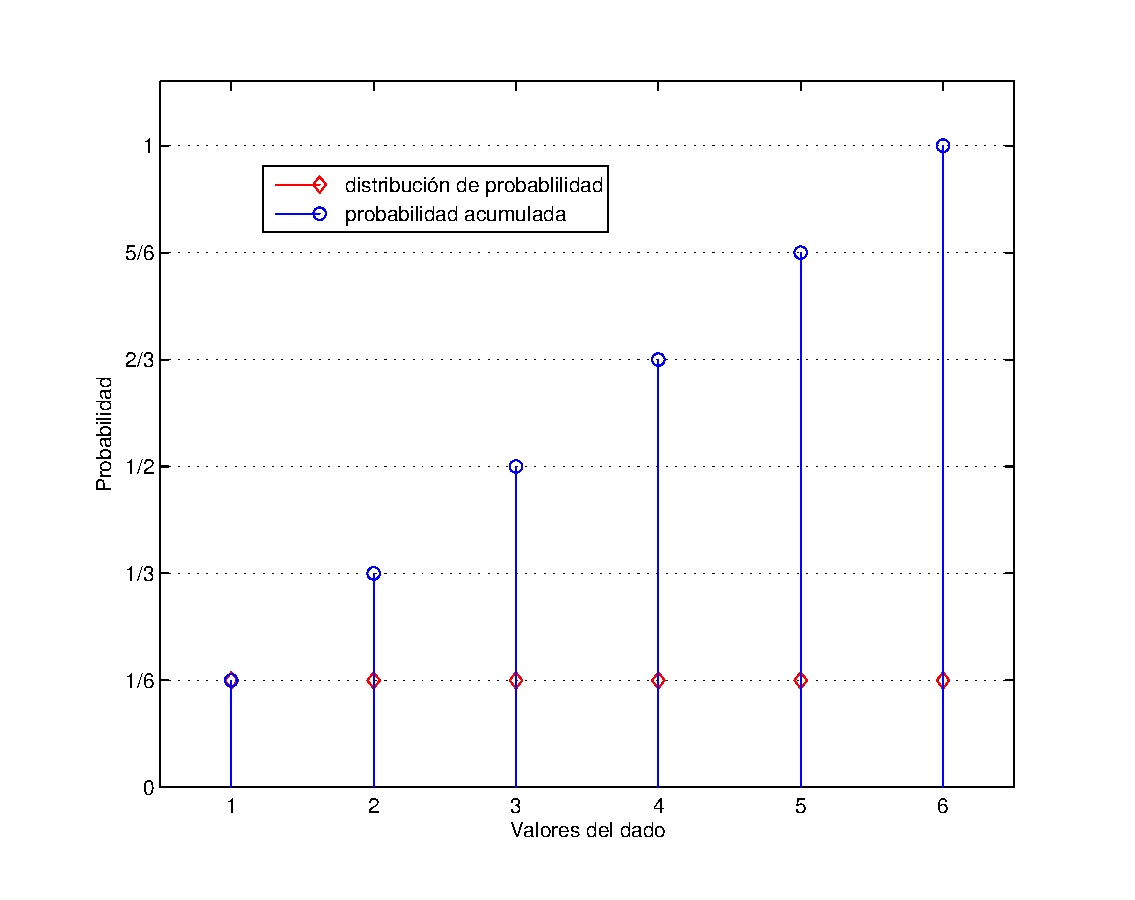
\includegraphics[width=10cm]{dado.eps}
\caption{Distribución de probabilidad y probabilidad acumulada de los resultados de lanzar un dado al aire.}
\label{fig:dado}
\end{figure}


Una propiedad que deben cumplir los sucesos aleatorios es que la suma de las probabilidades de todos los sucesos posibles debe ser igual a la unidad,

\begin{equation*}
\sum_{i=1}^n P(i) = 1
\end{equation*}

Es decir, \emph{necesariamente} debe darse alguno de los casos posibles.

Esto nos lleva al carácter aditivo o acumulativo de la probabilidad. Si elegimos un conjunto de casos posibles de un fenómeno aleatorio cualquiera, la probabilidad de que se de alguno de ellos será la suma de las probabilidades de los casos individuales. Por ejemplo la probabilidad al lanzar un dado de obtener un $2$, un $3$ ó un $6$ será,

\begin{equation*}
P(2,3,6) = P(2) + P(3) + P(6) = \frac{1}{6}+\frac{1}{6}+\frac{1}{6}=\frac{3}{6} = \frac{1}{2}
\end{equation*} 

lo que coincide con lo que intuitivamente cabía esperar, que la probabilidad de sacar uno cualquiera de los tres números fuera $0.5$.
La figura \ref{fig:dado} muestra la distribución de probabilidad y la probabilidad acumulada para el lanzamiento de un dado. La probabilidad acumulada guarda relación con el carácter aditivo de la probabilidad que acabamos de describir. Si consideramos el conjunto de valores posibles en orden: $1 < 2 < 3 < 4 < 5 < 6$, la probabilidad acumulada para cada valor es la probabilidad de sacar un número al lanzar el dado menor o igual que dicho valor. Así por ejemplo la probabilidad de sacar un número menor o igual que tres sería,

\begin{equation*}
P(n\leqslant 3) = P(1) + P(2) + P(3) = \frac{1}{6}+\frac{1}{6}+\frac{1}{6}=\frac{3}{6} = \frac{1}{2}
\end{equation*} 

Hasta ahora, todas las distribuciones discretas de probabilidad que hemos visto ---moneda, dado--- asignan la misma probabilidad a todos los sucesos posibles. En general esto no tiene porqué ser así. Supongamos un dado trucado en el que la probabilidad de sacar un $6$ valga $0.5$, es decir en promedio tiende a salir un $6$ la mitad de las veces que se lanza el dado. Supongamos además que todos los demás números salen con la misma probabilidad,
\begin{align*}
P(1)& = P(2) = P(3) = P(4) = P(5) = \frac{1}{10}\\
P(6)& = \frac{1}{2}\\
\sum_i P(i)& = 1 
\end{align*}

La figura \ref{fig:dadot} muestra la distribución de probabilidad y la probabilidad asociada al lanzamiento del dato trucado del ejemplo.
\begin{figure}
\centering
\includegraphics[width=10cm]{dadot.eps}
\caption{Distribución de probabilidad y probabilidad acumulada de los resultados de lanzar un dado trucado al aire.}
\label{fig:dadot}
\end{figure}


\subsection{Distribuciones de probabilidad continuas}\label{pdfc}
Hasta ahora, hemos considerado fenómenos en los que los casos posibles ---la variable aleatoria--- son finitos y numerables. Supongamos ahora un fenómeno aleatorio en que su variable aleatoria, $x$, es continua. Esto es: puede tomar todos los valores reales comprendidos en cierto intervalo, $x \in [a,b]$. Supongamos que todos los números contenidos en dicho intervalo pueden ser elegidos con igual probabilidad. Podríamos representar la distribución de probabilidad como una línea horizontal continua $f(x) = c$ que cubriera todo el intervalo $[a,b]$. Para obtener el valor constante $c$ de dicha distribución de probabilidad bastaría \emph{sumar} la probabilidad asociada por la distribución a cada valor del intervalo, igualar el resultado a uno y despejar $c$.

En realidad, no podemos sumar los infinitos valores que contiene el intervalo. De hecho lo que hacemos es sustituir la suma por una integral,

\begin{equation*}
\int_a^b c\cdot dx = 1 \Rightarrow c = \frac{1}{b-a}
\end{equation*}
\begin{figure}
\centering
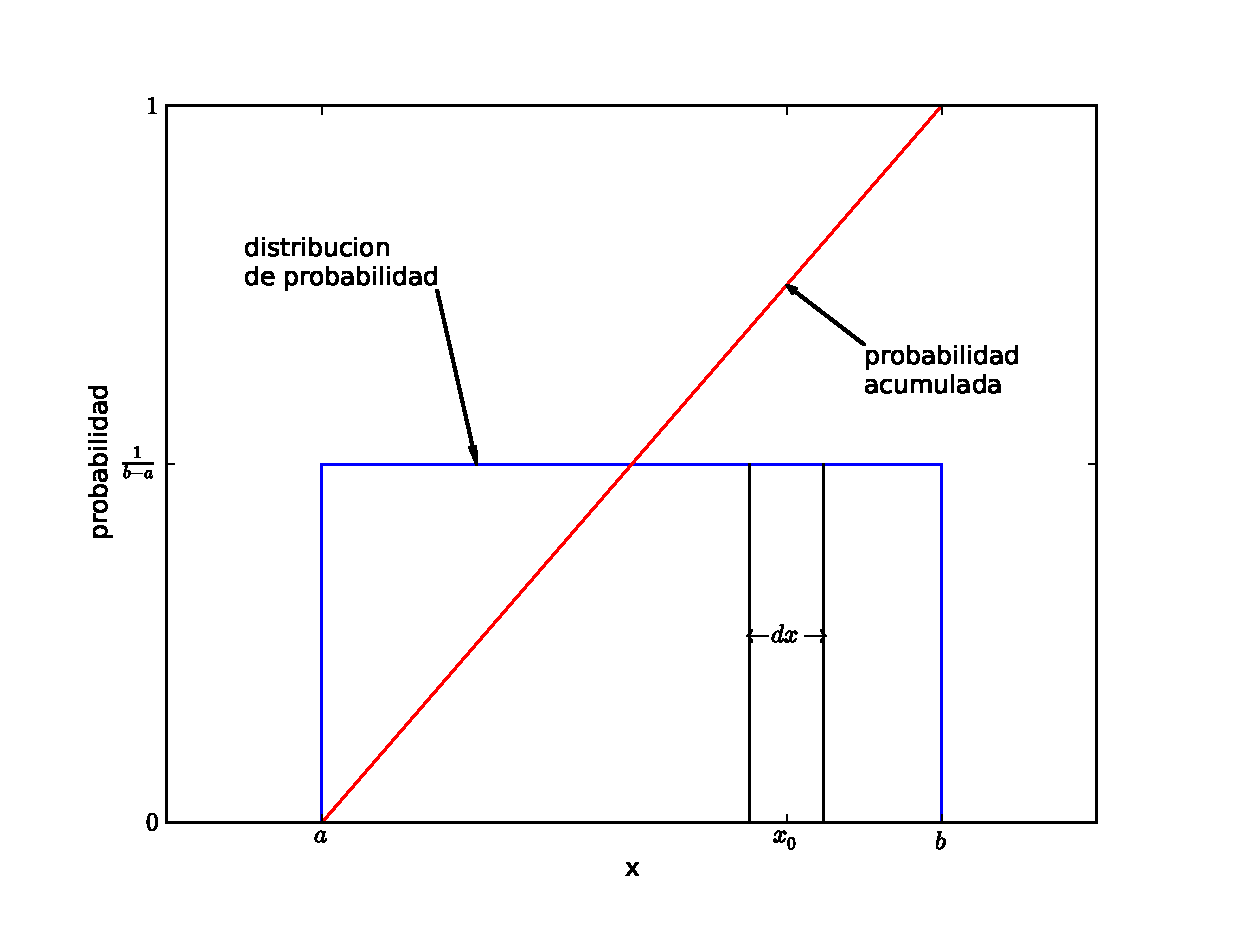
\includegraphics[width=10cm]{puniform.eps}
\caption{Distribución de probabilidad uniforme para un intervalo $[a,b]$ y probabilidad acumulada correspondiente}
\label{fig:puniform}
\end{figure}

La figura \ref{fig:puniform} muestra la distribución de probabilidad resultante

Es importante darse cuenta de la diferencia con el caso discreto. El intervalo $[a,b]$ contiene infinitos números. Si tratáramos de asignar un valor a la probabilidad de obtener un número dividiendo casos favorables entre casos posibles, como hacíamos en el caso discreto, obtendríamos un valor $0$ para todos los números. 

La distribución de probabilidad $f(x)\geqslant 0$ representa en el caso continuo una \emph{densidad} de probabilidad. Así, dado un número cualquiera $x_0 \in [a,b]$, el valor que toma la distribución de probabilidad $f(x_0)$ representa la probabilidad de obtener un número al azar en un intervalo $dx$ en torno a $x_0$,
\begin{equation*}
P\left(x_0-\frac{dx}{2}\leqslant x_0 \leqslant x_0+\frac{dx}{2}\right) = f(x_0)
\end{equation*} 

La probabilidad, vendrá siempre asociada a un intervalo, y se obtendrá integrando la distribución de probabilidad en dicho intervalo. Así por ejemplo,

\begin{equation*}
P(x_1 \leqslant x \leqslant x_2) = \int_{x_1}^{x_2}f(x)dx
\end{equation*}

representa la probabilidad de obtener un número al azar en intervalo $[x_1,x_2]$. 

La probabilidad acumulada, se obtiene también mediante integración, 

\begin{equation*}
P(x) = \int_a^xf(x)dx
\end{equation*}

Para el caso de la distribución de probabilidad constante descrita más arriba obtendríamos una línea recta que corta el eje de abcisas en $a$ y el valor de ordenada $1$ en b,
\begin{equation*}
P(x) = \int_a^xf(x)dx = \int_a^x \frac{1}{b-a}dx = \frac{x-a}{b-a}, \ x \in[a,b]
\end{equation*}
La figura \ref{fig:puniform} muestra la probabilidad acumulada para el ejemplo de la distribución uniforme. 

Si integramos la densidad de probabilidad sobre todo el intervalo de definición de la variable aleatoria, el resultado debe ser la unidad, puesto que dicha integral representa la probabilidad de obtener un número cualquiera entre todos los disponibles,

\begin{equation*}
\int_a^b f(x)dx =1, \ a\leqslant x \leqslant b
\end{equation*}

En probabilidad se emplean muchos tipos de distribuciones para representar el modo en que se dan los suceso aleatorios en la naturaleza. A continuación presentamos dos ejemplos muy conocidos:

\paragraph{Distribución exponencial} \index{Distribución exponencial}
La distribución exponencial está definida para sucesos que pueden tomar cualquier valor real positivo ó 0, $x \in [0,\infty)$. se representa mediante una función exponencial decreciente,
\begin{equation*}
f(x)=\frac{1}{\mu}e^{-\frac{x}{\mu}}
\end{equation*}

\begin{figure}
\centering
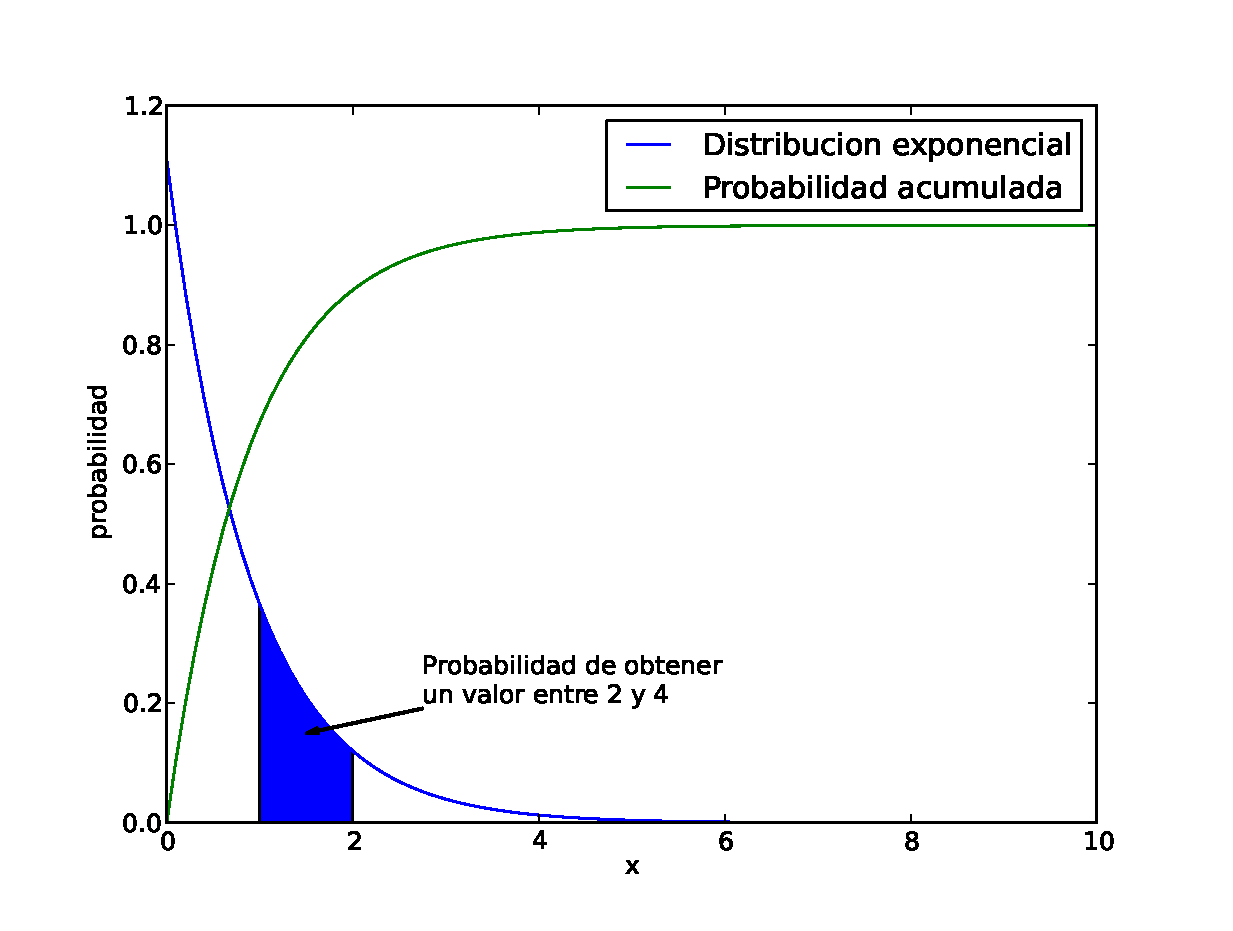
\includegraphics[width=10cm]{distexp.eps}
\caption{Distribución de probabilidad exponencial}
\label{fig:distexp}
\end{figure}

La figura \ref{fig:distexp} muestra un ejemplo de distribución exponencial. Es interesante observar como su probabilidad acumulada tiende a $1$ a medida que $x$ tiende a $\infty$.

\begin{equation*}
P(0\leqslant x < \infty) = \int_0^{\infty}\frac{1}{\mu}e^{-\frac{x}{\mu}}dx = 1
\end{equation*}

\paragraph{Distribución Normal}\index{Distribución normal} Aparece con gran frecuencia en la naturaleza. En particular, como veremos más adelante, está relacionada con la incertidumbre inevitable en la medidas experimentales. Esta definida para sucesos aleatorios que pueden tomar cualquier valor real, $-\infty < x < \infty$. Se representa mediante la función de Gauss,
\begin{equation*}
f(x)=\frac{1}{\sqrt{2\pi\sigma^2}}e^{-\frac{(x-\mu)^2}{2\sigma^2}}
\end{equation*}

La figura \ref{fig:normal} muestra un ejemplo de distribución normal.
\begin{figure}
\centering
\includegraphics[width=10cm]{normal.eps}
\caption{Distribución de probabilidad normal}
\label{fig:normal}
\end{figure}

\paragraph{Parámetros característicos de una distribución}

Los parámetros característicos permiten definir propiedades importantes de las distribuciones de probabilidad. Nos limitaremos a definir los dos más importantes:
\begin{itemize}\index{Media de una distribución}
\item \textbf{Media ó valor esperado.} El valor esperado de una distribución se obtiene integrando el producto de cada uno de los valores aleatorios sobre los que está definida la distribución, por su densidad de probabilidad,
\begin{equation*}
\mu = \int_a^b xf(x)dx, \ a\leqslant x \leqslant b
\end{equation*}

Así, para una distribución uniforme definida en un intervalo $[a,b]$,
\begin{equation*}
\mu = \int_a^b x\frac{1}{b-a}dx = \frac{a+b}{2}
\end{equation*}
para una distribución exponencial,
\begin{equation*}
\mu = \int_0^{\infty}x\frac{1}{\mu}e^{-\frac{x}{\mu}}dx = \mu
\end{equation*}
y para la distribución normal,
\begin{equation*}
\mu = \int_{-\infty}^{\infty}x \frac{1}{\sqrt{2\pi\sigma^2}}e^{-\frac{(x-\mu)^2}{2\sigma^2}}= \mu
\end{equation*}
Es interesante observar como en el caso de las distribuciones exponencial y normal la media es un parámetro que forma parte de la definición de la función de distribución.

\item \textbf{Varianza}\index{Varianza de una distribución} La varianza da una medida de la dispersión de los valores de la distribución en torno a la media. Se define como,
\begin{equation*}
\sigma^2 = \int_a^b (x-\mu)^2f(x)dx, \ a\leqslant x \leqslant b
\end{equation*}
Para una distribución uniforme definida en el intervalo $[a,b]$, tomará el valor,
\begin{equation*}
\sigma^2 = \int_a^b (x-\mu)^2\frac{1}{b-a}dx = \frac{(b-a)^2}{12}
\end{equation*}
para una distribución exponencial,
\begin{equation*}
\sigma^2 = \int_0^{\infty}(x-\mu)^2\frac{1}{\mu}e^{-\frac{x}{\mu}}dx = \mu^2
\end{equation*}
y para la distribución normal,
\begin{equation*}
\sigma^2 = \int_{-\infty}^{\infty}x \frac{1}{\sqrt{2\pi\sigma^2}}e^{-\frac{(x-\mu)^2}{2\sigma^2}}= \sigma^2
\end{equation*}

\item \textbf{Desviación estándar.} \index{Desviación estándar de una distribución} Es la raíz cuadrada de la varianza: $\sigma =\sqrt{\sigma^2}$  
\end{itemize}

\section{El teorema del límite central}\label{tlc}

El teorema del límite central juega un papel muy importante a la hora de analizar y evaluar resultados experimentales. Nos limitaremos a enunciarlo, pero no daremos una demostración.

Supongamos que tenemos un fenómeno aleatorio continuo que viene caracterizado por una variable aleatoria $x$. Además el fenómeno aleatorio viene descrito por una distribución de probabilidad arbitraria $f(x)$ de media $\mu$ y varianza $\sigma^2$.

Supongamos que realizamos un experimento consistente en obtener $n$ valores de x al azar. Los valores así obtenidos, deberán seguir la distribución de probabilidad $f(x)$. Para caracterizar nuestro experimento, calcularemos la media de los $n$ valores obtenidos,

\begin{equation*}
\bar{x}_n=\frac{1}{n}\sum_{i=1}^n x_i
\end{equation*}

Si repetimos el experimento muchas veces, obtendremos al final una colección de medias; tantas, como veces hemos repetido el experimento,
$\left\{\bar{x}_{n1}, \bar{x}_{n2} \cdots \bar{x}_{nj} \cdots \right\}$. El teorema del límite central, establece que las medias así obtenidas constituyen a su vez valores de una variable aleatoria que sigue una distribución normal, cuya media coincide con la media $\mu$ de la distribución original $f(x)$ y cuya varianza coincide con el valor de la varianza de la distribución original $\sigma^2$ dividida por el número $n$ de valores de $x$ obtenidos al azar en cada uno de los experimentos. (En todos los experimentos se obtiene siempre el mismo número de valores de la variable aleatoria $x$).

\begin{equation*}
x, \ f(x), \mu, \sigma^2 \Rightarrow \bar{x}_n,\ f(\bar{x}_n)=\frac{1}{\sqrt{2\pi\sigma^2/n}}e^{-\frac{(x-\mu)^2}{2\sigma^2/n}}  
\end{equation*}

Veamos un ejemplo para ilustrar el teorema. Hemos visto en la sección \ref{rand} que el comando \texttt{rand} de Matlab genera números aleatorio uniformemente distribuidos en el intervalo\footnote{En realidad es el intervalo $[2^{-52},1-2^{-52}]$ podemos considerarlo equivalente al intervalo $(0,1)$ debido a la precisión finita de los números máquina} $(0,1)$. Podemos considerar que el ordenador genera número aleatorios que siguen aproximadamente una distribución continua en dicho intervalo. Podemos alterar dicho intervalo multiplicando el resultado de \texttt{rand} por un número cualquiera. Así, por ejemplo,
\begin{verbatim}
>> x=5*rand(100)
\end{verbatim} 
genera un vector de 100 números aleatorios en el intervalo $(0,5)$.
Además podemos desplazar el centro del intervalo sumando o restando al resultado anterior un segundo número. Así,

\begin{verbatim}
>> x =5*rand(100) -2
\end{verbatim}
genera un vector de 100 números aleatorios en el intervalo $(-2,3)$.

Para comprobar el teorema del límite central, podemos construir un bucle que genere un vector de $n$ números aleatorios en un determinado intervalo, calcule su media y guarde el resultado en un vector de medias. El siguiente código de Matlab, realiza dicho cálculo primero generando un vector de $10$ números aleatorios ($n = 10$) y después generando un vector de $100$, ($n=100$).  El programa genera en cada caso un millón de vectores distintos.
%\begin{lstlisting}
%% Este código genera un millón de vectores, formados por números 
%% aleatorios distribuidos uniformemente en el intervalo (-1,1).
%% Calcula el valor medio de los valores de cada vector y guarda
%% el resultado en un nuevo vector.
%
%media10 = zeros(1,1000000); % vector para guardar las medias
%for i=1:1000000
% 	media10(i) = mean(2*rand(10,1)-1);
%end
%
%% se repite el mismo calculo pero ahora con vectores de 100
%% elementos
%media100 = zeros(1,1000000)
%for i=1:1000000
%	medias100(i) = mean (2*rand(100,1)-1);
%end	
%\end{lstlisting}s

De acuerdo con el teorema del límite central, los dos vectores de medias obtenidos, \texttt{media10} y \texttt{media100}, deben seguir distribuciones normales tales que,
\begin{enumerate}
\item La media de la distribución normal debe coincidir con la media de la distribución a la que pertenecían los datos originales. Como hemos tomado datos distribuidos uniformemente en el intervalo $[-1,1]$, La media de dicha distribución es,
\begin{equation*}
\mu = \frac{(b+a)}{2}=\frac{1+(-1)}{2}=0
\end{equation*}
\item La varianza de las distribuciones normales a las que pertenecen las medias obtenidas será en cada caso el resultado de dividir la varianza de la distribución uniforme original entre el número de datos empleados para calcular dichas medias,


\begin{align*}
\sigma_{10}^2 = \frac{\sigma^2}{10}=\frac{\frac{(b-a)^2}{12}}{10}=\frac{\frac{(1-(-1))^2}{12}}{10}=\frac{1}{30}\\
\sigma_{100}^2 = \frac{\sigma^2}{100}=\frac{\frac{(b-a)^2}{12}}{100}\frac{\frac{(1-(-1))^2}{12}}{10}=\frac{1}{300}
\end{align*}s
\end{enumerate}

\begin{figure}
\centering
\begin{subfigure}{0.35\textwidth}
	{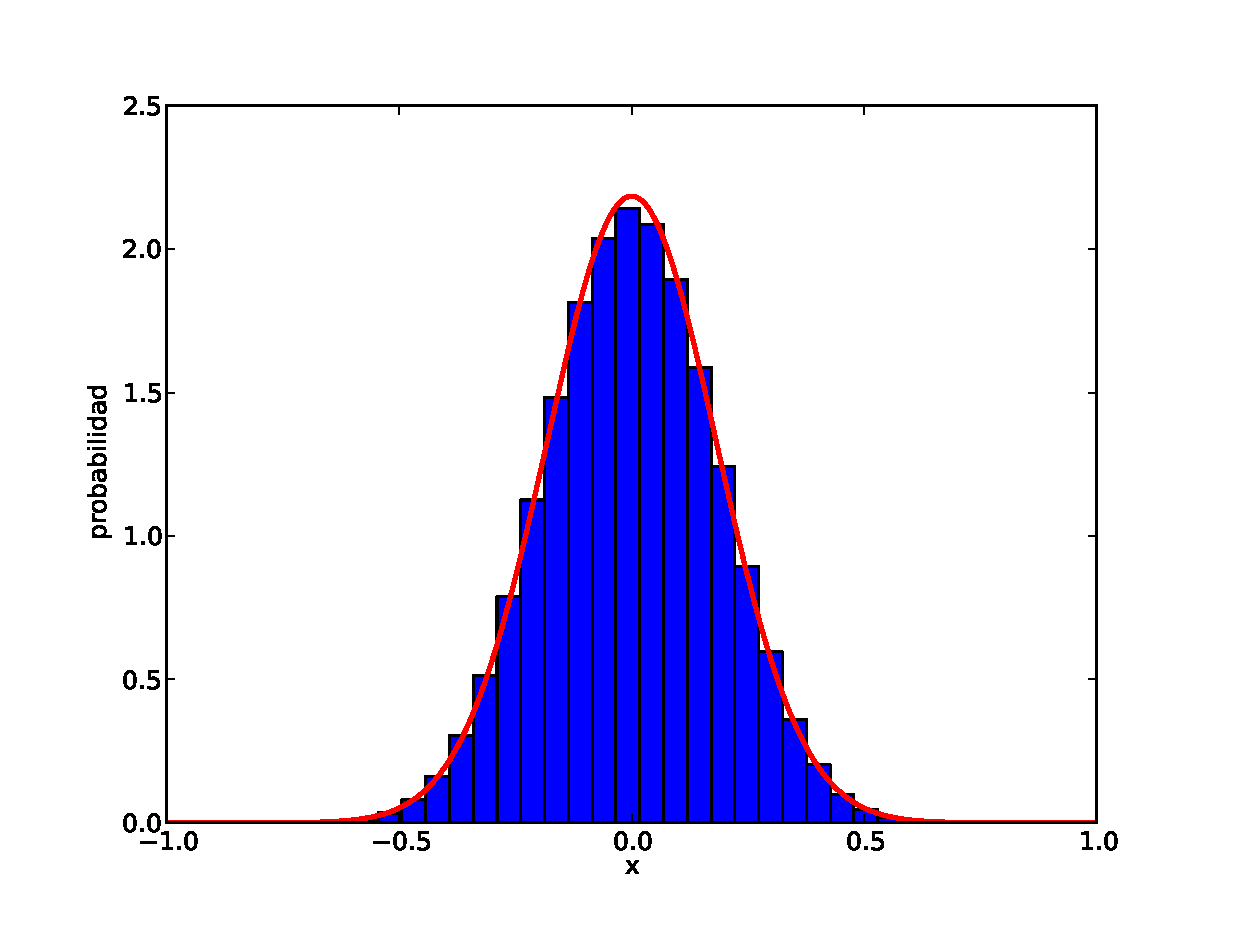
\includegraphics[width=\textwidth]{tlc1.eps}}
\caption{Distribución para medias de 10 valores}\label{fig:tlc10}
\end{subfigure} 
\begin{subfigure}{0.35\textwidth}
	{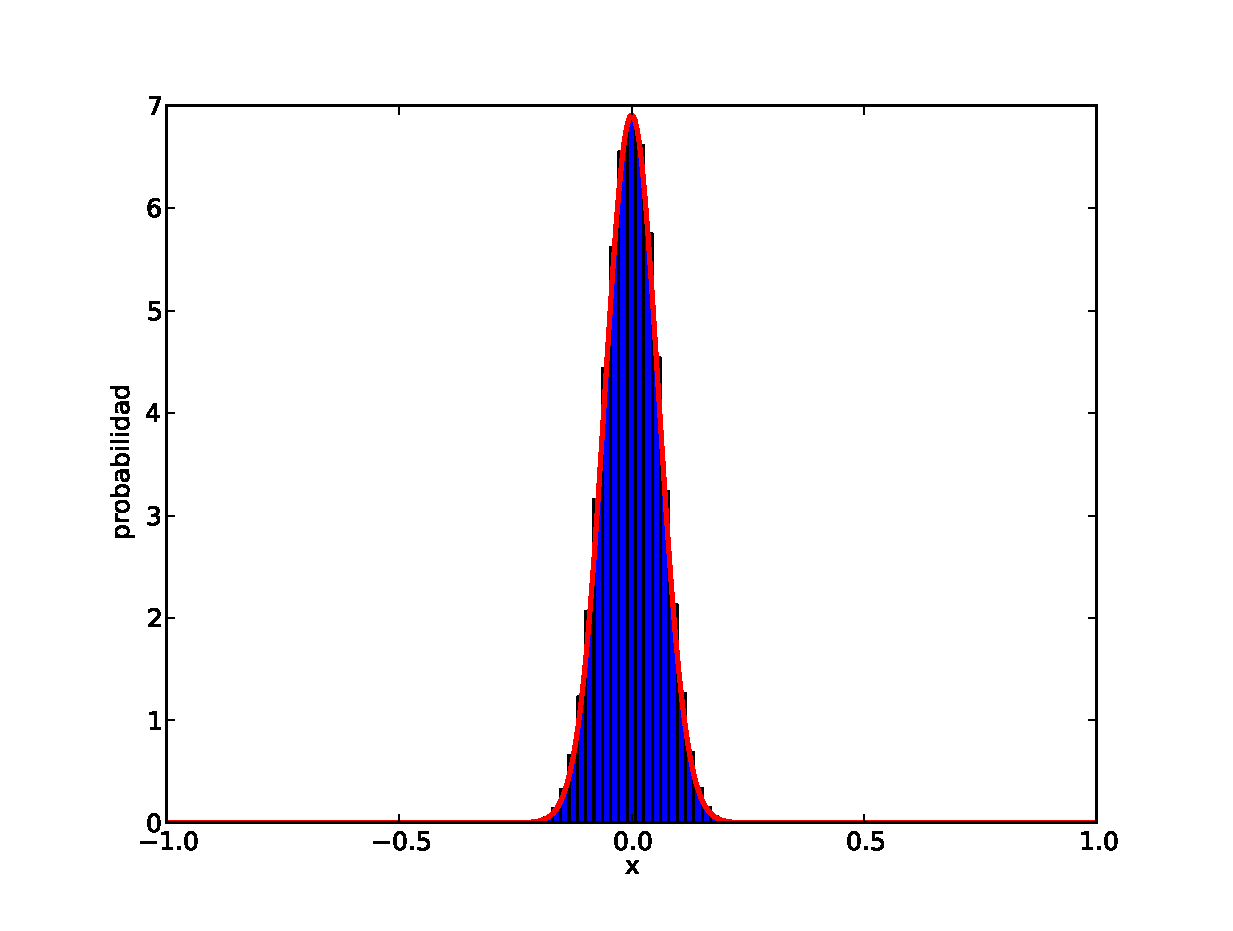
\includegraphics[width=\textwidth]{tlc2.eps}}
	\caption{Distribución para medias de 100 valores}  \label{fig:tlc100}
\end{subfigure}
\caption{Teorema del límite central: Comparación entre histogramas normalizados para un millón de medias y la distribución normal a que pertenecen}
\end{figure}


Por tanto, las distribuciones normales a las que pertenecen las medias calculadas son,


\begin{equation*}
f(\bar{x}_{10})=\frac{1}{\sqrt{2\pi\frac{1}{30}}}e^{-\frac{(x-\mu)^2}{2\frac{1}{30}}},\  f(\bar{x}_{100})=\frac{1}{\sqrt{2\pi\frac{1}{300}}}e^{-\frac{(x-\mu)^2}{2\frac{1}{300}}}
\end{equation*}

Las figuras \ref{fig:tlc10} y \ref{fig:tlc100}, muestran un histograma normalizado de las medias obtenidas con el código que acabamos de describir \footnote{El histograma normalizado se obtiene dividiendo el número de puntos que pertenecen a cada barra del histograma entre el número total de puntos y el ancho de la barra. De esta manera, si sumamos los valores representados en cada barra multiplicados por su ancho, el resultado es la unidad. Solo normalizando el histograma es posible compararlo con la distribución a que pertenecen los datos, que cumple por definición tener área unidad.}. Sobre dicho histograma se ha trazado mediante una línea roja, la función de Gauss que representa en cada caso la distribución normal a que pertenecen las medias. Como puede observarse en ambos casos el histograma normalizado y la distribución coinciden bastante bien.

De las figuras, es fácil deducir que cuantos más datos empleemos en el cálculo de las medias, más centrados son los resultados obtenidos en torno a la media de la distribución original. Por otro lado, esto es una consecuencia lógica del hecho de que la varianza de la distribución normal que siguen las medias, se obtenga dividiendo la varianza de la distribución original, por el número de datos $n$; cuantos mayor es $n$ más pequeña resulta la varianza de la distribución normal resultante.
 
\section{Incertidumbre en las medidas experimentales}
Siempre que realizamos una medida de una cantidad física dicha medida  estará afectada por un cierto error. Dado que no conocemos cual es el valor verdadero que toma la magnitud que estamos midiendo, no podemos tampoco conocer el error que cometemos al medirla. Decimos entonces que toda medida está afectada por un cierto grado de incertidumbre.

Lo que sí es posible hacer, es acotar el grado de incertidumbre de una medida, es decir estimar unos límites con respecto a la medida realizada dentro de los cuales debe estar contenido el verdadero valor que toma la magnitud medida.

Cualquier medida experimental debe incluir junto al resultado de la medida el valor de su incertidumbre y, por supuesto, las unidades empleadas en la medida. La figura \ref{fig:incertidumbre} muestra un modo correcto de expresar una medida experimental, aunque no es el único. Como puede observarse, la medida y su incertidumbre se separan en la representación mediante el símbolo $\pm$.  La incertidumbre se representa como  un entorno alrededor del valor medido, dentro del cual estaría incluido el valor real de la medida\footnote{Como se verá más adelante se debe indicar también el \emph{grado de confianza} con el que esperamos que la medida caiga dentro del intervalo indicado por la incertidumbre}. 

\begin{figure}
\centering
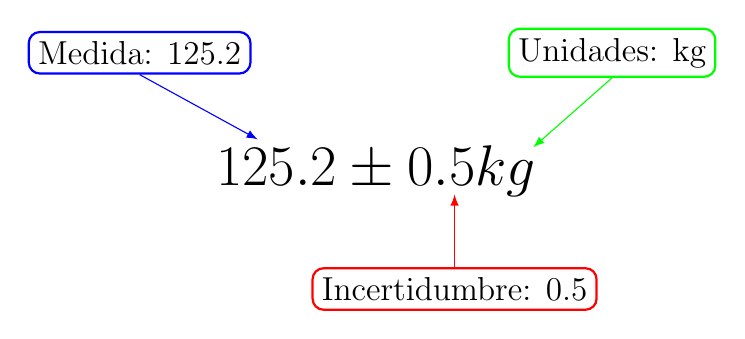
\begin{tikzpicture}
%\usetikzlibrary{shapes.geometric}
\path (3,0) node(a) [rectangle,draw=blue, thick,rounded corners,align=center,font=\large]{Medida: $125.2$}
(7,-3) node(b)[rectangle,draw=red, thick,rounded corners,align=center,font=\large]{Incertidumbre: $0.5$}
(9,0) node(c)[rectangle,draw=green, thick,rounded corners,align=center, font=\large]{Unidades: kg}
(6,-1.5) node(d)[font= \huge]{$125.2 \pm 0.5 \text{kg}$};
\draw[blue,-latex](a.south)--(4.5,-1.1);
\draw[red,-latex](b.north)--(7,-1.8);
\draw[green,-latex](c.south)--(8.0,-1.2);
\end{tikzpicture}
\caption{Modo correcto de expresar una medida experimental}
\label{fig:incertidumbre}
\end{figure} 

 
\subsection{Fuentes de incertidumbre.}

Antes de entrar en el estudio de las fuentes de incertidumbre, es importante destacar que el estudio de la medición constituye por sí mismo una ciencia, conocida con el nombre de metrología. Lo que vamos a describir a continuación tanto referido a las fuentes de incertidumbre como al modo de estimarla, es incompleto y representa tan solo una primera aproximación al problema.
La incertidumbre de una medida tiene fundamentalmente dos causas:

\paragraph{Incertidumbre sistemática de precisión.}\index{Medidas experimentales! precisión}
 La primera es la precisión limitada de los aparatos de medida. Cualquier aparato de medida tiene una precisión que viene determinada por la unidad o fracción de unidad más pequeña que es capaz de resolver. Por ejemplo, una regla normal, es capaz de resolver (distinguir) dos longitudes que se diferencien en $0.5 mm$, un reloj digital sencillo es capaz de resolver tiempos con una diferencia de $1s.$ etc.
La incertidumbre debida a la precisión finita de los aparatos de medida recibe el nombre de \emph{Incertidumbre sistemática de precisión.} 
Se llama así porque depende exclusivamente de las características del aparato de medida que, en principio, son siempre las mismas.

La incertidumbre sistemática de precisión suele expresarse añadiendo a la medida la mitad de la división mínima de la escala del aparato de medida empleado. Así, por ejemplo, si medimos $123 mm$ con una regla graduada en milímetros, podríamos expresar la  medida como $123 \pm 0.5 mm$ o también como $12,3\pm0.05cm$.


La incertidumbre sistemática de precisión representa una distribución uniforme de media el valor de la medida realizada y anchura la división mínima de la escala. Es decir, se considera que el valor real de la medida está dentro de dicho intervalo intervalo con una probabilidad del $100\%$. Volviendo al ejemplo anterior de la regla, el valor real de nuestra medida estaría comprendido en el intervalo $[122.5,\ 123.5 ]$, y podría tomar cualquier valor de dicho intervalo con igual probabilidad. 

\paragraph{Incertidumbre estadística.} La segunda fuente de incertidumbre se debe a factores ambientales, que modifican de una vez para otra las condiciones en que se realiza una medida experimental. Estos factores hacen que la medidas realizadas sean sucesos aleatorios. En principio podría describirse mediante una distribución de probabilidad $f(x)$, pero en la práctica desconocemos de qué distribución se trata y ni siquiera sabemos cual es su valor esperado $\mu$ o su varianza $\sigma$. \index{Medidas experimentales! Incertidumbre estadística}

Afortunadamente, el teorema del límite central, que describimos en al sección \ref{tlc} proporciona un sistema de estimar la incertidumbre estadística.

Supongamos que repetimos $n$ veces la misma medida experimental. Por ejemplo: tenemos un recipiente con agua, lo calentamos y tomamos la temperatura del agua cuando ésta rompe a hervir. Repetimos $n$ veces el experimento y obtenemos un conjunto $\{x_1,x_2,\cdots x_n \}$ de medidas de la temperatura de ebullición del agua. Cabe esperar que, debido a la incertidumbre estadística, los valores obtenidos sean distintos  y, a la vez próximos entre sí\footnote{De hecho, si aparecen algunos valores claramente alejados del resto, lo habitual es considerar que están afectados por algún error desconocido y desecharlos. Dichos valores suelen recibir el nombre de valores o datos aberrantes.}.

Sabemos que dichos valores deben seguir una cierta distribución de probabilidad. Podríamos estimar su valor esperado $\mu$ mediante el cálculo de la media aritmética de las medidas tomadas.
\begin{equation*}
\mu \approx \bar{x}_n = \frac{1}{n}\sum_{i=1}^n x_i
\end{equation*}

La media así calculada se toma como el valor resultante de la medida realizada.

De acuerdo con el teorema del límite central, $\bar{x}_n$ es una variable aleatoria que debe seguir una distribución normal de media $\mu$ y de varianza $\sigma^2/n$. Como tampoco conocemos el valor de la varianza $\sigma^2$ de la distribución de probabilidad que siguen los datos medidos, la estimamos a partir de los propios datos medidos, de acuerdo con la siguiente ecuación,
\begin{equation*}
\sigma^2 \approx s^2 = \frac{1}{n-1}\sum_{i=1}^n(x_i-\bar{x})^2
\end{equation*}

Dividiendo $s^2$ por el número de muestras empleado se puede aproximar la varianza de la distribución normal que debe seguir $\bar{x}_n$,

\begin{equation*}
\sigma^2_{xn} \approx s^2_{xn} = \frac{s^2}{n}
\end{equation*}

La incertidumbre, se puede asociar con la raíz cuadrada la varianza que acabamos de estimar,

\begin{equation*}
s_{xn}=\sqrt{s^2_{xn}}=\sqrt{\frac{\frac{1}{n-1}\sum_{i=1}^n(x_i-\bar{x})^2}{n}}
\end{equation*}

esta cantidad recibe el nombre de desviación estándar.

\subsection{Intervalos de confianza.}
Como hemos visto, a partir del teorema central del límite podemos asociar la media de los valores obtenidos al repetir una medida y su desviación estándar con una distribución normal. Podemos ahora, en un segundo paso,s asociar la incertidumbre de la medida realizada con la probabilidad representada por dicha distribución normal.

Si el valor obtenido tras realizar $n$ repeticiones de una medida es $\bar{x}_n$ y su desviación típica es $s_{xn}$ ¿Cuál es la probabilidad de que el valor medido esté realmente comprendido en el intervalo $[\bar{x}_n-s_{xn}, \bar{x}_n+s_{xn}]$? 

Como vimos en el apartado \ref{pdfc}, dicha probabilidad puede calcularse integrando la distribución normal obtenida entre $\bar{x}_n-s_{xn}$ y $\bar{x}_n+s_{xn}$,

\begin{equation*}
P(\bar{x}_n - s_{xn} \leqslant x \leqslant \bar{x}_n
+ s_{xn}) = \frac{1}{\sqrt{2\pi\sigma^2_{xn}}}\int_{\bar{x}_n-s_{xn}}^{\bar{x}_n+s_{xn}}e^{\frac{-(x-\bar{x}_n)^2}{2s_{xn}^2}}
\end{equation*}
\begin{figure}[h]
\centering
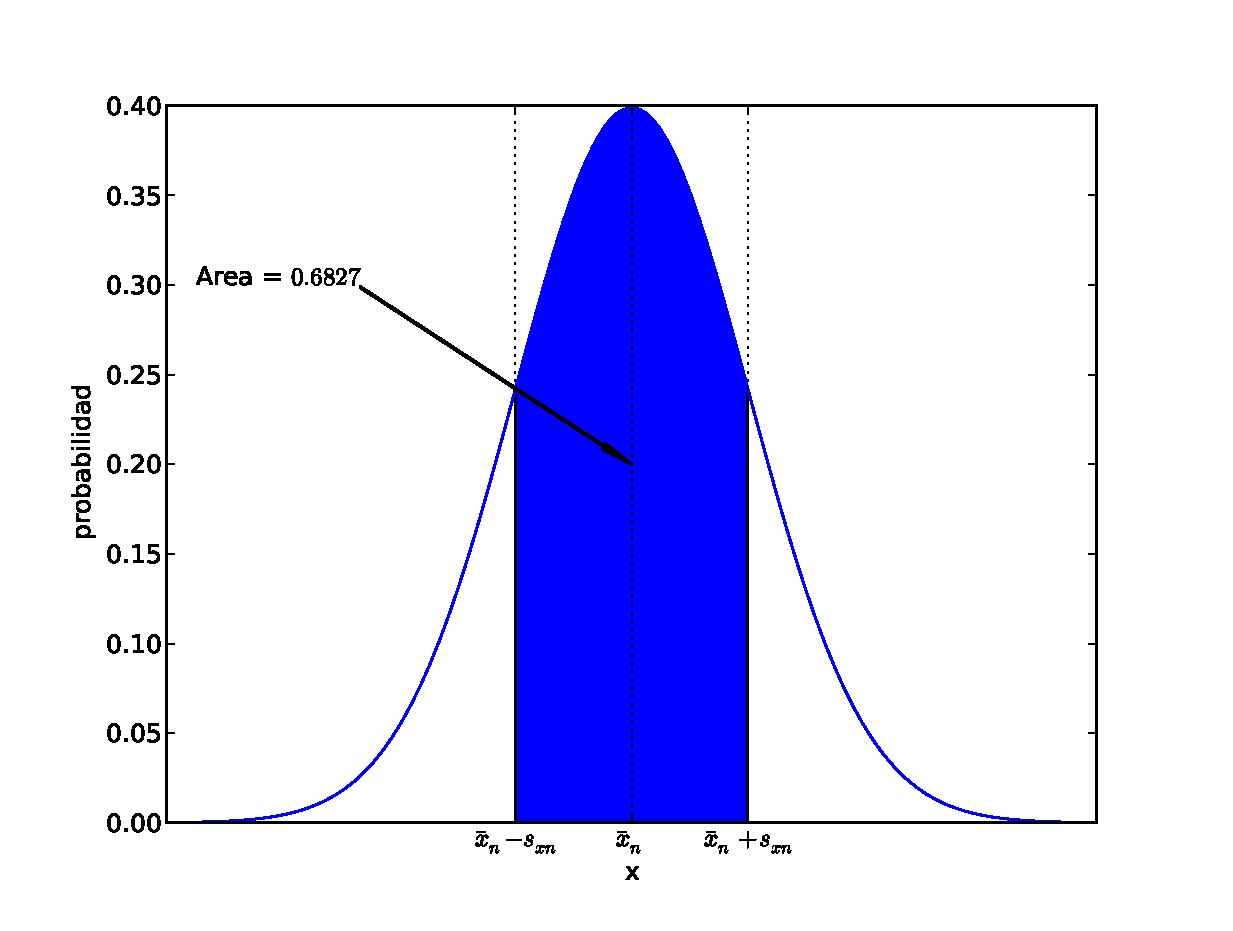
\includegraphics[width=10cm]{interconf1.eps}
\caption{Intervalo de confianza del $68.27\%$ }
\label{fig:ic1}
\end{figure}

El valor de dicha integral es $0.6827$. Si expresamos este valor como un tanto por ciento, concluimos que la probabilidad de que el valor medido este en el intervalo $[\bar{x}_n-s_{xn}, \bar{x}_n+s_{xn}]$ es del $68.27\%$. Dicho de otra manera: el intervalo $[\bar{x}_n-s_{xn}, \bar{x}_n+s_{xn}]$ corresponde con el \emph{intervalo de confianza} del 68.27\%. La figura \ref{fig:ic1} muestra el área bajo la distribución normal, correspondiente a dicha probabilidad.

Volviendo al problema de la medida, la manera correcta de expresarla sería en nuestro caso:  $\bar{x}\pm s_{xn}$ (unidades). Indicando que la incertidumbre corresponde con el intervalo de confianza del $68.27\%$.


Observando la figura \ref{fig:ic1}, es fácil plantearse la siguiente cuestión: ¿Qué valor de la incertidumbre contendría el valor de real de la medida con una probabilidad de, por ejemplo, el 95\%? O, dicho de otra manera, ¿Cuánto tengo yo que \emph{alargar} el intervalo de integración para que el área contenida bajo la distribución normal valga $0.95$?

Para estimarlo se emplea la inversa de la función de probabilidad acumulada. Como se explicó en el apartado \ref{pdfc}, la función de probabilidad acumulada se obtiene por integración de la distribución de probabilidad correspondiente. 

Dicha función representa la probabilidad de obtener un resultado entre el límite inferior para el que está definida la distribución de probabilidad y el valor $x$ para el que se calcula la función. La inversa de la función de probabilidad acumulada nos indica, dado un valor de la probabilidad comprendido entre $0$ y $1$, a qué valor $x$ corresponde dicha probabilidad acumulada. 

Dado que la distribución normal no tiene primitiva, solo puede integrarse numéricamente. Por tanto, su inversa, solo puede obtenerse también numéricamente. Matlab, suministra la función \texttt{norminv(p)}, que permite obtener directamente los valores de la inversa de la función de probabilidad normal acumulada.

Además, la función \texttt{norminv(p)} calcula la función de probabilidad inversa acumulada para una distribución de probabilidad normal de media $0$ y varianza $1$. En realidad esto no supone ningún problema ya que para obtener el valor correspondiente a cualquier otra distribución normal, basta multiplicar el valor $x$ obtenido con \texttt{norminv(p)} por el valor de la desviación estándar y sumarle el valor de la media de la distribución deseada.

Antes de seguir adelante, veamos algunos ejemplos de uso de esta función. Por ejemplo si introducimos en la función el valor $0.1$,
\begin{verbatim}
>> p = 0.1;
>> x = norminv(p)s
>> x = -1.2815515655446004
\end{verbatim}

Es decir la probabilidad de obtener un número en el intervalo $(-\infty, -1.2815515655446004]$ vale $0.1$ o, lo que es equivalente, un 10\%.

Otro ejemplo especialmente significativo: Si introducimos el valor $0.5$, 

\begin{verbatim}
>> p = 0.5;
>> x = norminv(p)
>> x = 0.0
\end{verbatim}

Como cabría esperar de la simetría de la distribución normal, hay un $0.5$ ---50\%--- de probabilidades de obtener un número entre $-\infty$ y $0$.  La figura \ref{fig:invcum} muestra la función inversa de probabilidad acumulada y en particular el punto  correspondiente al valor 0.5.

\begin{figure}[h]
\centering
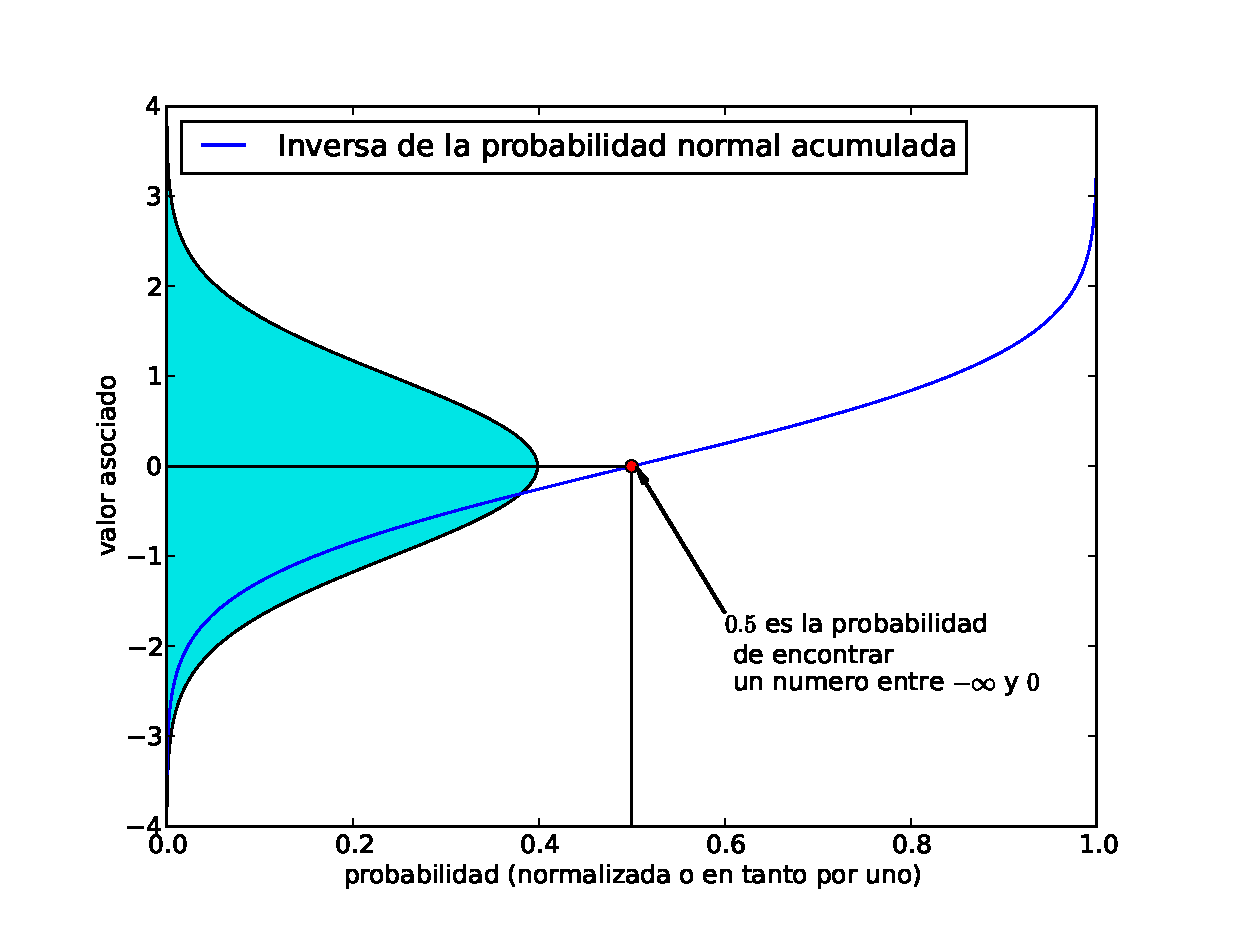
\includegraphics[width=10cm]{invcum.eps}
\caption{Función inversa  de probabilidad normal acumulada}
\label{fig:invcum}s
\end{figure}

Supongamos ahora que queremos repetir el cálculo para una distribución normal de media $\mu=6$ y desviación típica $\sigma = 2$. Para el valor $0.1$ obtendríamos,

\begin{verbatim}
>> p = 0.1;
>> x = norminv(p)
>> x = -1.2815515655446004
>> mu = 6
>> sigma = 2
>> x2 = sigma*x+mu
>> x2 = -1.5631031310892007
\end{verbatim}

Por tanto, ahora tenemos un 10\% de probabilidades de obtener un número entre $-\infty$ y $-1.5631031310892007$

Retomando el hilo de nuestro problema, lo que a nosotros realmente nos interesa, es encontrar intervalos de confianza, es decir conocer el intervalo en torno al valor medio $\bar{x}_n$ que corresponde a una determinada probabilidad. La función inversa de probabilidad acumulada nos da el intervalo entre $-\infty$ y $x$ correspondiente a una determinada probabilidad. Si combinamos los resultados de dicha función con las propiedades de simetría y área unidad de la función normal podemos obtener el intervalo centrado en torno a la media correspondiente a una determinada probabilidad.

Así el intervalo $[-x ,x]$ correspondiente a  una probabilidad del $P\%$, abarca un área bajo la curva $P/100$. Por tanto el área que queda en las colas ---a derecha e izquierda del intervalo--- es $1-x/100$. Como la distribución normal es simétrica, dicha área debe dividirse en dos, una correspondiente a la cola $[-\infty, -x]$ y la otra correspondiente a la cola $[x, \infty]$.

\begin{figure}[h]
\centering
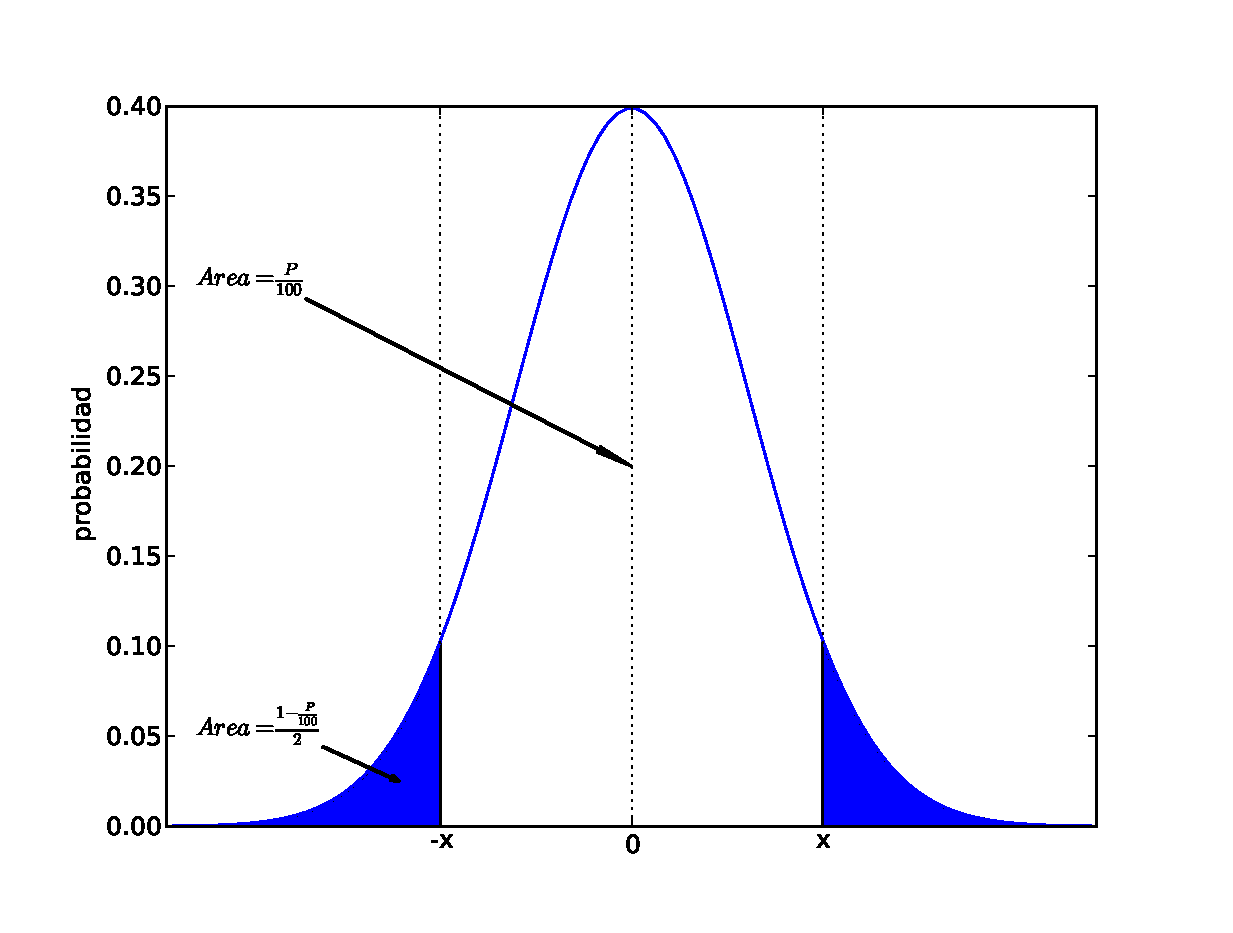
\includegraphics[width=10cm]{intervalo.eps}
\caption{Intervalo de probabilidad P\%}
\label{fig:intervalo}
\end{figure}
La figura \ref{fig:intervalo} muestra gráficamente la relación de áreas que acabamos de describir; las dos colas aparecen pintadas en azul. 


Para obtener el límite inferior, $-x$, del intervalo de probabilidad $P\%$ basta emplear la función \texttt{norminv}, introduciendo como variable de entrada el área de la cola, \texttt{x=norminv((1-P/100)/2)}. Así por ejemplo, para obtener el límite inferior del intervalo de confianza correspondiente a una probabilidad del $90\%$,

\begin{verbatim}
>> p=(1-0.90)/2
p =
    0.0500

>> x=norminv(p)
x =
   -1.6449
\end{verbatim}

Por tanto el intervalo de confianza correspondiente a una probabilidad del $90\%$ para una distribución normal de media cero y desviación estándar uno es, $I_{90\%} =[-1.6449\ 1.6449]$

Supongamos ahora que hemos realizado un conjunto de $n$ medidas de una determinada magnitud física, por ejemplo temperatura en ºC, y obtenemos su media $\bar{x}_n=6.5$ ºC y su desviación estándar $s_{xn}=2$. Si queremos dar el resultado de la medida con una incertidumbre correspondiente a un intervalo de confianza del $95\%$, calculamos el intervalo de confianza empleando la función inversa de probabilidad acumulada normal, y después, multiplicamos el resultado por $s_{xn}$ para ajustarlo a la distribución normal que sigue la media de nuestros datos, 

\begin{verbatim}
>> xm = 6; %media de las medidas
>> sigma = 2; %desviacion de las medidas
>> p = (1-0.95)/2 % probabilidad acumulada hasta limite inferior del intervalo
p =
    0.0250
>> i95 = norminv(p) % limite inferior del intervalo
i95 =
   -1.9600 
>> incert = i95*sigma %limite inferior de la incertidumbre
incert =
   -3.9199
\end{verbatim}

Por tanto, en este ejemplo, debemos expresar la medida como $6.5 \pm 3.92$ ºC indicando que el intervalo de confianza es del $95\%$.

\paragraph{La distribución T de Student.} Habitualmente, cuando el número de medidas que se han tomado para estimar el valor de $\bar{x}_n$ es pequeño, los intervalos de confianza se calculan empleando la distribución t de Student de n-1 grados de libertad, donde  n representa el número de medidas tomadas.

\begin{figure}[h]
\centering
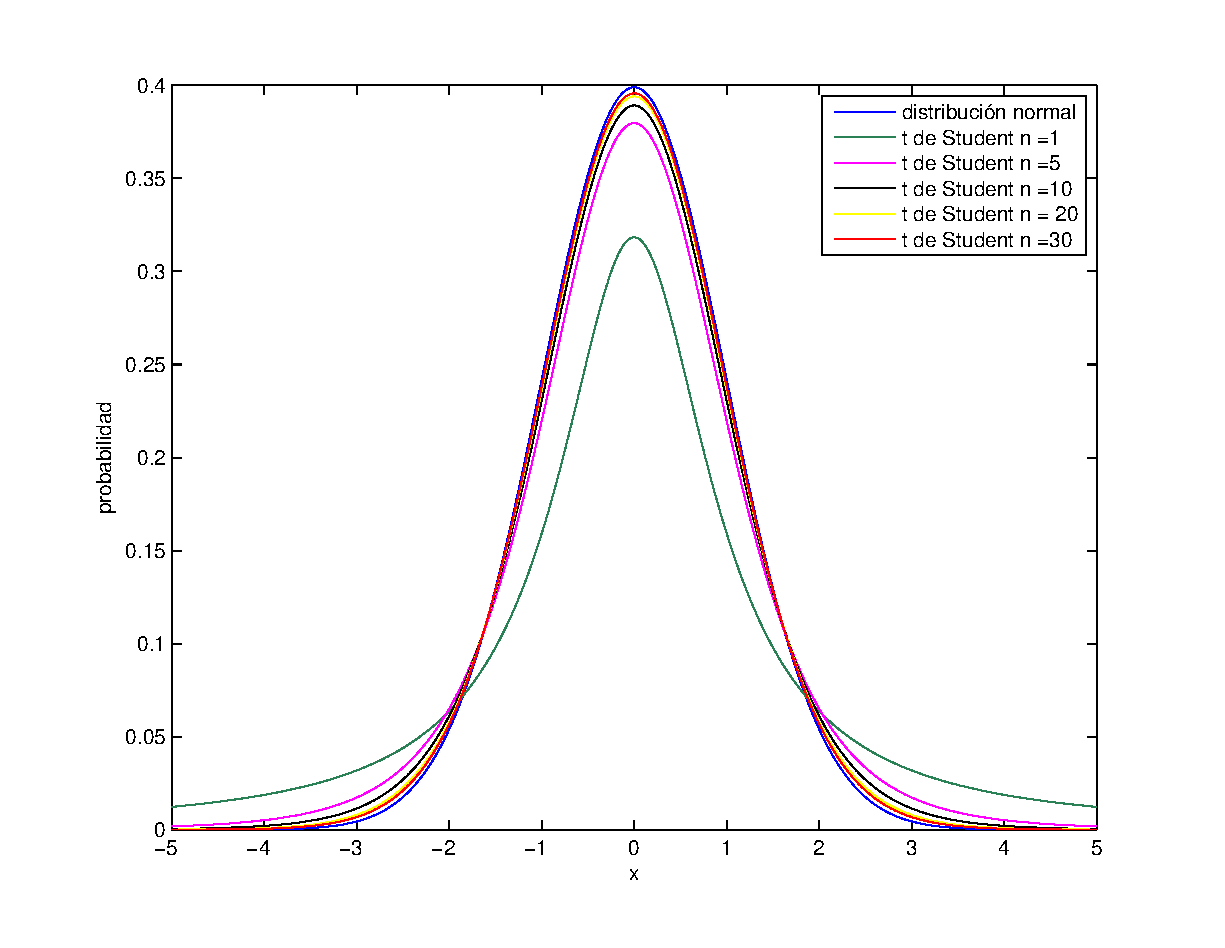
\includegraphics[width=10cm]{tdestudent.eps}
\caption{Comparación entre las distribuciones t de Student de 1, 5, 10, 20 y 30 grados de libertad y la distribución normal.}
\label{fig:tdst}
\end{figure}

Para un número pequeño de muestras, la distribución t de Student da una aproximación mejor que la distribución normal. Para un número de muestras grande, ambas distribuciones son prácticamente iguales.  La figura \ref{fig:tdst} muestra una comparación entre la distribución normal y la distribución t de Student, calculada para distintos grados de libertad. De la figura se puede concluir en primer lugar que la desviación estándar de la distribución t de Student es en todos los casos mayor que la de la distribución normal, con lo cual los intervalos de confianza para un valor dado de la probabilidad son siempre mayores. En segundo lugar se observa también que para 30 o más medidas --- $n\geqslant 30$ --- la diferencia entre las distribuciones t de Student y normal es prácticamente despreciable.

El procedimiento de cálculo es el mismo que si empleamos la distribución normal, basta sustituir la inversa de la distribución normal acumulada por la inversa de la distribución t de Student acumulada. En Matlab, esta función esta definida como: \texttt{x = tinv(p,n)}. 

Así, para el ejemplo anterior de las medidas de temperatura de media  $\bar{x}_n=6.5$ ºC y  desviación estándar $s_{xn}=2$  si suponemos que el número de medidas tomadas es $n=5$. El intervalo de confianza correspondiente a un $95\%$  lo calcularíamos mediante la inversa de la distribución de probabilidad t de Student de $n-1$ grados de libertad acumulada como,

\begin{verbatim}
>> xm = 6; %media de las cinco medidas
>> sigma = 2; %desviacion de las cinco medidas
>> p = (1-0.95)/2 % probabilidad acumulada hasta limite inferior del intervalo
p =
    0.0250
>> i95 = tinv(p,4) % limite inferior del intervalo 4 =5-1 grados de libertad para cinco medidas
i95 =
   -2.7764
>> incert = i95*sigma %limite inferior de la incertidumbre
incert =
   -5.5529
\end{verbatim}

Por tanto deberíamos expresar el valor de la medida realizada como, $6.5\pm 5.55$ ºC. Si comparamos este resultado con el obtenido empleando la distribución normal, vemos que el intervalo de confianza y, por tanto, la incertidumbre han aumentado.

\subsection{Propagación de la incertidumbre: Estimación de la incertidumbre de medidas indirectas.}

Supongamos que deseamos obtener la incertidumbre de una determinada magnitud física $y$ que no hemos medido directamente, sino que se determina a partir de otras cantidades $x_1,x_2,\cdots,x_n$ empleando una relación funcional $f$,

\begin{equation*}
y = f(x_1,x_2,\cdots,x_n)
\end{equation*}

La función $f$ suele recibir el nombre de ecuación de medida, y no tiene por qué representar simplemente una ley física; de hecho, debería incluir entre sus entradas cualquier cantidad que pueda contribuir a modificar significativamente la incertidumbre de $y$. Por ejemplo: diferentes observadores, laboratorios, experimentos, horas a las que se han realizado las observaciones, etc.

La incertidumbre asociada al valor de $y$, a la que llamaremos $u_c(y)$, se expresa en función de la desviación estándar de $y$,  

\begin{equation*}
u_c(y) =\sqrt{s_c^2(y)}
\end{equation*}


donde  $s_c^2(y)$ se define como la  varianza \emph{combinada} de $y$, que se estima en primera aproximación a partir de la expansión en serie de Taylor\footnote{En primera aproximación empleamos un desarrollo de Taylor de primer orden. En realidad, lo adecuado o no de este método depende de las características de la función $f$. No discutiremos aquí este problema.} de la función $f$	

\begin{equation*}
s_c^2(y) = \sum_{i=1}^n\left(\frac{\partial f}{\partial x_i}\right)^2 s^2(x_i) + 2\sum_{i=1}^{n-1}\sum_{i=1}^n \frac{\partial f}{\partial x_i}\frac{\partial f}{\partial x_j} c_v(x_i,x_j)
\end{equation*}

Donde $s^2(x_i)$  representa la varianza asociada a la entrada $x_i$ y $c_v(x_i, x_j)$ la covarianza entre las entradas $x_i$ y $x_j$. 

La covarianza entre dos variables $z$ y $t$ de las que se tienen $n$ muestras, puede estimarse a partir de las muestras como,

\begin{equation*}
c_v(z,t) =\frac{1}{n-1}\sum_{i=1}^n(z_i-\bar{z})(t_i-\bar{t})
\end{equation*}

De modo análogo a como hicimos en el caso de la varianza de la media de un conjunto de medidas, podemos relacionar la covarianza entre las medias de  de dos variables, con la covarianza entre $n$ medidas de dichas variables como,

\begin{equation*}
c_v(\bar{z},\bar{t}) =\frac{c_v(z,t)}{n}
\end{equation*}

En muchos casos de interés no existe correlación entre las variables de entrada. En estos casos, los valores de la covarianza será nulos y podemos simplificar la ecuación empleada en el cálculo de $s_c^2(y)$,

\begin{equation*}
s_c^2(y) = \sum_{i=1}^n\left(\frac{\partial f}{\partial x_i}\right)^2 s^2(x_i)
\end{equation*}


Un ejemplo simple lo podemos obtener de la ecuación para la potencia disipada en una resistencia eléctrica. En este caso, el valor de la potencia disipada depende del voltaje, $V$, de la resistencia $R_0$ medida a una temperatura de referencia $t_0$, de la temperatura real a que se encuentra la resistencia $t$ y, en primera aproximación, de un coeficiente que $b$, que establece una relación linea entre temperatura y resistencia. 

\begin{equation*}
P = f(V,R_o,b,t) = \frac{V^2}{R_0\left(1+b(t-t_0)\right)}
\end{equation*}

Supongamos que $b$ es un coeficiente numérico no sujeto a incertidumbre y que las  variables $V$, $R_0$, $t$ y $t_0$ no están correlacionadas entre sí. Podemos entonces expresar la varianza  en la  potencia disipada, a partir de las varianzas de las variables de entrada como,

\begin{equation*}
s_c^2(P) = \left(\frac{\partial f}{\partial V}\right)^2 s^2(V)+ \left(\frac{\partial f}{\partial R_0}\right)^2 s^2(R_0)+ \left(\frac{\partial f}{\partial t}\right)^2 s^2(t)+\left(\frac{\partial f}{\partial t_0}\right)^2 s^2(t_0)    
\end{equation*}

Por tanto,

\begin{align*}
s_c^2(P) =& \left(\frac{2V}{R_0\left(1+b(t-t_0)\right)}\right)^2 s^2(V)+ \left(\frac{-V^2\left(1+b(t-t_0)\right)}{R_0^2\left(1+b(t-t_0)\right)^2}\right)^2 s^2(R_0)+\\
&+ \left(\frac{-V^2R_0b}{R_0^2\left(1+b(t-t_0)\right)^2}\right)^2 s^2(t)+\left(\frac{V^2R_0b}{R_0^2\left(1+b(t-t_0)\right)^2}\right)^2 s^2(t_0)    
\end{align*}

y la incertidumbre en la potencia disipada será la raíz cuadrada de la expresión que acabamos de obtener: $u_c(P) =\sqrt{s_c^2(P)} $

Establecer los intervalos de confianza, para una incertidumbre propagada no es tan sencillo como en el caso de una incertidumbre obtenida directamente de una medida experimental. En primera aproximación, podemos suponer que $y$ sigue una distribución normal de media el valor obtenido, a partir de la función $f$ y desviación $u_c(p)$ y estimar los intervalos de confianza del mismo modo que se describió anteriormente para una medida directa.  Pero esto no es siempre correcto. No podemos establecer en realidad ninguna ley general que relacione las distribuciones de probabilidad de las incertidumbres de las variables de entrada con la distribución de probabilidad de la incertidumbre de la variable de salida.

\subsection{Ejemplo de estimación de la incertidumbre con Matlab.}

Para aclarar los métodos descritos en los apartados anteriores, vamos obtener la incertidumbre de la potencia disipada en una resistencia, siguiendo la ecuación descrita en el apartado anterior . La tabla \ref{tabres} muestras los datos obtenidos tras realizar 20 medidas experimentales de la tensión y la temperatura en una resistencia.

\begin{table}[h]
\caption{Mediciones de temperatura y Voltaje, sobre una resistencia de prueba de 100 $\Omega$}
\label{tabres}
\centering
\begin{tabular}{cccc}
\hline
Valor nominal de la resistencia& $R_0=100 \pm 5 \Omega$ (intervalo confianza 98\%) \\ 
\hline
Temperatura de referencia& $t_0=50\pm 0.1 ^oC$ (división menor del sensor $0.2^oC$) \\
\hline
Valor del parámetro b& $b = 0.4\Omega / ^oC$ (incertidumbre despreciable)\\
\hline
\hline
Temperatura ºC& Votaje mV\\
\hline
 $55.7$&$761$\\
\hline 
 $62.8$&$897$\\
\hline 
 $58.1$&$879$\\
\hline 
 $60.9$&$767$\\
\hline 
 $66.3$&$758$\\
\hline 
 $59.4$&$763$\\
\hline 
 $61.8$&$762$\\
\hline 
 $62.5$&$761$\\
\hline 
 $59.4$&$790$\\
\hline 
 $61.4$&$852$\\
\hline 
 $55.7$&$816$\\
\hline 
 $65.3$&$752$\\
\hline 
 $56.9$&$848$\\
\hline 
 $57.8$&$920$\\
\hline 
 $62.9$&$743$\\
\hline 
 $59.9$&$858$\\
\hline 
 $62.6$&$761$\\
\hline 
 $59.1$&$788$\\
\hline 
 $57.9$&$775$\\
\hline
 $53.8$&$791$\\
\hline
\hline
\end{tabular}
\end{table}

Para obtener la incertidumbre en el valor de la potencia disipada por la resistencia debemos en primer lugar calcular la varianza de las medidas directas suministradas en la tabla.

\begin{itemize} 

\item Varianza del valor nominal de la resistencia $R_0$: En este caso, la tabla nos suministra como dato el intervalo de confianza correspondiente al 98\%.  Podemos emplear la función de Matlab \texttt{nominv(x)} para calcular la desviación estándar de $R_0$. Como hemos visto, el límite inferior del intervalo de confianza del 98 \%, corresponde con una probabilidad acumulada de $(1-0.98)/2$,
\begin{verbatim}
>> i98 = norminv((1-0.98)/2)
i98 =
   -2.3263
\end{verbatim} 

Dicha cantidad, multiplicada por la desviación estándar de $R_0$, corresponde con el limite inferior del intervalo de confianza suministrado en la tabla  para $R_0$. Por tanto,

\begin{verbatim}
>> sR0 =-5/i98  %desviación estandar de R0
sR0 =
    2.1493
>> s2R0 =sR0^2  %varianza de R0
s2R0 =
     4.6195
\end{verbatim}

luego $s^2(R_0)= 4.6195$

\item Varianza de la temperatura de referencia $t_0$: En este caso se ha expresado la incertidumbre en función de la mitad de la división más pequeña de la escala del aparato de medida. Podemos considerar por tanto que la incertidumbre estaría representada por una distribución uniforme definida en el intervalo $[-0.1\ 0.1]$. En esta caso, podemos asociar la varianza de la medida directamente con dicha distribución uniforme, 

\begin{verbatim}
>> s2t0=(1-(-1))^2/12
s2t0 =
    0.3333
\end{verbatim}

Así, $s^2(t_0)=0.3333$

\item Varianzas de las medidas de temperatura y voltaje:
En primer lugar promediamos los valores  obtenidos de voltaje y temperatura, para calcular el valor de la medida. Matlab tiene definida la función \texttt{mean(x)} que permite obtener directamente el valor medio de los elementos de \texttt{x}. Podemos por tanto definir en Matlab dos vectores, unos para los datos de temperatura y otro para los datos de voltaje y calcular directamente las medias,

\begin{verbatim}
>> t=[55.7 62.8 58.1 60.9 66.3 59.4 61.8 62.5 59.4 61.4 55.7 65.3 56.9 57.8 62.9...
59.9 62.6 59.1 57.9 53.8]

t =

  Columns 1 through 6
   55.7000   62.8000   58.1000   60.9000   66.3000   59.4000
  Columns 7 through 12
   61.8000   62.5000   59.4000   61.4000   55.7000   65.3000
  Columns 13 through 18
   56.9000   57.8000   62.9000   59.9000   62.6000   59.1000
  Columns 19 through 20

   57.9000   53.8000
>> v=[761 897 879 767 758 763 762 761 790 852 816 752 848 920 743 858 761...
 788 775 791]

v =

  Columns 1 through 10
   761   897   879   767   758   763   762   761   790   852
  Columns 11 through 20
   816   752   848   920   743   858   761   788   775   791

>> tm =mean(t)
tm =
   60.0100

>> vm =mean(v)
vm =
  802.1000
\end{verbatim}

Una vez estimadas las medias, que emplearemos como valores de las medidas de la temperatura y el voltaje,  podemos ahora estimar la varianza o la desviación estándar de las medias haciendo uso de las función de Matlab \texttt{std(x)}, para la desviación estándar,  y de \texttt{var(x)}, para la varianza.  Además, debemos aplicar el teorema central del límite, dividiendo por el número de datos disponible.

\begin{verbatim}
>> s2t=var(t)/length(t) %varianza de la temperatura media
s2t =
    0.5328
>> s2t=var(v)/length(v) %varianza del voltaje medio

s2t =
  145.5837
 >> st=std(v)/sqrt(length(v)) %desviacion del voltaje medio
st =
   12.0658

>> st=std(t)/sqrt(length(t)) %desviacion de la temperatura media
st =
    0.7300
\end{verbatim} 

Lógicamente, los resultados muestran que las desviaciones estándar son las raíces cuadradas de las varianzas. Tenemos por tanto, $\bar{t}=60.01$, $\bar{V}=802,01$, $s^2(t)=0.5382$, $s^2(V)=145.5837$.

\end{itemize} 

En este momento, hemos reunido ya toda la información necesaria para estimar la incertidumbre de la potencia consumida en la resistencia de nuestro ejemplo. La tabla \ref{tabdatos} contiene los datos calculados,

\begin{table}[h]
\caption{Medidas y varianzas estimadas}
\label{tabdatos}
\centering
\begin{tabular}{cccc}
\hline
Variable (unidades) & Valor & Varianza  \\ 
\hline
\hline
$R_0$($\Omega$)&$100$&$4.6195$\\
\hline
b ($\Omega$/ºC)& $0.4$ &--\\
\hline
$t_0$ (ºC)& 50& 0.3333\\
\hline 
 $\bar{t}$ (ºC)&$60.01$&$0.5328$\\
\hline 
$\bar{V}$(mV)& $802.01$&$145.5837$\\
\hline
\hline
\end{tabular}
\end{table}

Podemos ahora calcular la potencia,

\begin{equation*}
P = \frac{V^2}{R_0\left(1+b(t-t_0)\right)}=\frac{0.80201^2}{100\left(1+0.4(60.01-50)\right)} =  0.001285 W = 1.285 mW
\end{equation*}

Donde hemos introducido el voltaje en voltios, para  obtener la potencia directamente en vatios.

A continuación, propagamos la incertidumbre de las variables de entrada a la de salida,

\begin{align*}
s_c^2(P) =& \left(\frac{2V}{R_0\left(1+b(t-t_0)\right)}\right)^2 s^2(V)+ \left(\frac{-V^2\left(1+b(t-t_0)\right)}{R_0^2\left(1+b(t-t_0)\right)^2}\right)^2 s^2(R_0)+\\
&+ \left(\frac{-V^2R_0b}{R_0^2\left(1+b(t-t_0)\right)^2}\right)^2 s^2(t)+\left(\frac{V^2R_0b}{R_0^2\left(1+b(t-t_0)\right)^2}\right)^2 s^2(t_0)=\\
=& \left(\frac{2 \cdot 0.80201}{100\left(1+0.4(60.01-50)\right)}\right)^2 \cdot 1.455836\cdot10^{-4} + \left(\frac{- 0.80201^2\left(1+0.4(60.01-50)\right)}{100^2\left(1+0.4(60.01-50)\right)^2}\right)^2 \cdot 4.619+\\
&+ \left(\frac{- 0.80201^2\cdot100\cdot0.4}{100^2\left(1+0.4(60.01-50)\right)^2}\right)^2\cdot 0.5328 +\left(\frac{0.80201^2\cdot100\cdot0.4}{100^2\left(1+0.4(60.01-50)\right)^2}\right)^2 0.3333=\\
=&1.4959\cdot10^{-09} + 7.6327\cdot10^{-10} + 5.6252\cdot10^{-09} + 3.5189\cdot10^{-09} =  1.1403\cdot 10^{-08}
\end{align*} 

En este caso, hemos multiplicado la varianza del voltaje $s^2(V)$ por $10^{-6}$, para obtener $s_c^2(P)$ en W$^2$. Podemos expresar ahora la incertidumbre de la potencia consumida en función de la desviación estándar como,

\begin{equation*}
u_c(P) = \sqrt{s_c^2(P)} =  1.0678\cdot 10^{-4} W
\end{equation*}

Con lo que finalmente expresaríamos la medida indirecta de la potencia consumida como, $P = 1.285 \pm 0.10678 $ mW. Si suponemos que la distribución de probabilidad asociada a la incertidumbre de la potencia es normal, la incertidumbre así expresada (mediante la desviación estándar) representaría un intervalo de confianza del $68.27\%$. 

